% !TeX document-id = {182a71a9-0e53-4007-bbd0-360f73891856}
% !TeX TXS-program:compile = txs:///latexmk/{}[-xelatex -synctex=1 -interaction=nonstopmode]

%\documentclass[UTF8,openright,12pt,]{ctexbook}  %When you need to print the pdf ,choose this one. If it still can't satisfied you, you may turn to Cover and reconsitution/reconsitution.tex .I'm sure it will.
\documentclass[openany,12pt]{ctexbook} %When you want to submit the pdf , then choose this one.

% !TeX root = ../Main/XMU.tex
\usepackage{ctex}
\ctexset{today=big,}
\usepackage{amssymb}
\usepackage{amsmath,amsthm}
\usepackage{amsfonts}
\usepackage{verbatim}
\usepackage{ifthen}
\usepackage{xcolor}
\usepackage{multirow}
\usepackage{longtable}
\usepackage[para]{threeparttable}
\usepackage{array,booktabs,longtable,tabularx}
\usepackage[font={small,bf}]{caption}
\usepackage{setspace}
\usepackage{subfigure}

\usepackage[a4paper,
%bindingoffset=1cm,
left=2.5cm,
right=2.5cm,
top=3cm,
bottom=4cm,
footskip=1.5cm,
twoside,
]{geometry}

\usepackage{graphicx}
\graphicspath{{../Figures/}}%设定图片的存放路径
\usepackage{tikz}
\newcommand*\circled[1]{\tikz[baseline=(char.base)]{
		\node[shape=circle,draw,inner sep=1pt] (char) {#1};}}
\usepackage{pifont}
\renewcommand\thefootnote{\ding{\numexpr171+\value{footnote}}} %改变注脚的格式

%设置代码的插入
\usepackage{listings}
\def\lstbasicfont{\fontfamily{pcr}\selectfont\footnotesize}
\lstset{%
	numbers=left,
	numberstyle=\tiny,
	basicstyle=\small,
	backgroundcolor=\color{white},      % choose the background color
	basicstyle=\footnotesize\ttfamily,  % size of fonts used for the code
	columns=fullflexible,
	tabsize=4,
	breaklines=true,               % automatic line breaking only at whitespace
	captionpos=b,                  % sets the caption-position to bottom
	commentstyle=\color{green},  % comment style
	escapeinside={\%*}{*)},        % if you want to add LaTeX within your code
	keywordstyle=\color{blue},     % keyword style
	stringstyle=\color{purple}\ttfamily,  % string literal style
	frame=single,
	rulesepcolor=\color{red!20!green!20!blue!20},
}
\lstloadlanguages{C,C++,Java,Matlab,Mathematica}

%算法的插入宏包
\usepackage{algorithm}
\usepackage[noend]{algpseudocode}

\makeatletter
\def\BState{\State\hskip-\ALG@thistlm}
\makeatother


%font
\usepackage{fontspec}
\usepackage{xeCJK}%中文字体
%Windows请保留以下三行代码。而Mac用户请注释以下三行代码,开启后面三行代码。Linux用户请自行配置字体。
% \setCJKmainfont[ItalicFont={楷体}, BoldFont={黑体}]{宋体}%衬线字体 缺省中文字体为
% \setCJKsansfont{黑体}
% \setCJKmonofont{楷体}%中文等宽字体

\setCJKmainfont[ItalicFont={Kai}, BoldFont={Hei}]{STSong}%衬线字体 缺省中文字体为
\setCJKsansfont{Hei}
\setCJKmonofont{Kai}%中文等宽字体

\setmainfont{Times New Roman} %西文部分默认使用的字体
\setsansfont{Times New Roman} %西文默认无衬线字体
\setmonofont{Times New Roman}%西文默认的等宽字体

\usepackage[super]{gbt7714}
\usepackage[sort&compress]{natbib}
\renewcommand{\citep}[1]{{\color{blue}\citeauthor{#1}(\citeyearpar{#1})}}

\usepackage{fancyhdr}
\fancyhf{}
\fancyhead[CE]{\xiaowu \sffamily  \xmutitle}
\fancyhead[CO]{\xiaowu \sffamily  \CTEXthechapter\quad \leftmark}
\fancyfoot[C]{\thepage}
%\lhead{\textnormal{\kaishu\leftmark}}
%\chead{\textnormal{\kaishu\rightmark}}
%\rhead{--\ \thepage\ --}
%\pagestyle{fancy}

\usepackage[bookmarks=true,bookmarksnumbered=false,
colorlinks,linkcolor=black,
citecolor=blue,urlcolor=green]{hyperref}
\usepackage{cleveref}
%\let\oldeqref\eqref
%\renewcommand{\eqref}{公式}\oldeqref}

\crefname{figure}{图}{}
\crefname{table}{表}{}
\crefname{equation}{公式}{}
%equation, chapter, section, etc.
%\creflabelformat{htypei}{hformati}
\newtheorem{theory}{定理}[section]
\theoremstyle{definition}\newtheorem{law}{定律}[section]
\def\lq{`}\def\rq{'}


%%%%%%%%%%%%%%%%%%%%%%%%%%%%%%%%%%%%%%%%%%%%%%%%%%%%%%%%%%%
% 重定义字号命令
%%%%%%%%%%%%%%%%%%%%%%%%%%%%%%%%%%%%%%%%%%%%%%%%%%%%%%%%%%%
\newcommand{\xiaochu}{\fontsize{30pt}{40pt}\selectfont}    % 小初, 1.5倍行距
\newcommand{\yihao}{\fontsize{26pt}{36pt}\selectfont}    % 一号, 1.4倍行距
\newcommand{\erhao}{\fontsize{22pt}{28pt}\selectfont}    % 二号, 1.25倍行距
\newcommand{\xiaoer}{\fontsize{18pt}{18pt}\selectfont}    % 小二, 单倍行距
\newcommand{\sanhao}{\fontsize{16pt}{24pt}\selectfont}    % 三号, 1.5倍行距
\newcommand{\xiaosan}{\fontsize{15pt}{22pt}\selectfont}    % 小三, 1.5倍行距
\newcommand{\sihao}{\fontsize{14pt}{21pt}\selectfont}    % 四号, 1.5倍行距
\newcommand{\banxiaosi}{\fontsize{13pt}{19.5pt}\selectfont}    % 半小四, 1.5倍行距
\newcommand{\xiaosi}{\fontsize{12pt}{18pt}\selectfont}    % 小四, 1.5倍行距
\newcommand{\dawuhao}{\fontsize{11pt}{11pt}\selectfont}    % 大五号, 单倍行距
\newcommand{\wuhao}{\fontsize{10.5pt}{10.5pt}\selectfont}    % 五号, 单倍行距
\newcommand{\xiaowu}{\fontsize{9pt}{9pt}\selectfont}    % 小五号, 单倍行距





\makeatletter

\newcommand\Dotfill{\leavevmode\cleaders\hb@xt@ .68em{\hss .\hss }\hfill\kern\z@}

% for chapter
\newcommand\@chaplable[1]{第\zhnumber{#1}章}
\renewcommand\chapter{\if@openright\cleardoublepage\else\clearpage\fi
%	\thispagestyle{fancy}
	\global\@topnum\z@
%	\@afterindentfalse
	\secdef\@chapter\@schapter}
\renewcommand\@chapter[3][default]{%
	\ifnum \c@secnumdepth >\m@ne
	\if@mainmatter
	\refstepcounter{chapter}%
	\typeout{第\thechapter 章}%
	\addcontentsline{toc}{chapter}%
	{\protect\numberline{\@chaplable{\thechapter}}\hspace{-2.5em}#1 \Dotfill }%
	\addcontentsline{eoc}{chapter}%
	{\protect\numberline{\chaptername\ \thechapter }\hspace{-1.8em}#3 \Dotfill }%
	\else
	\addcontentsline{toc}{chapter}{#1}%
	\addcontentsline{eoc}{chapter}{#3}%
	\fi
	\else
	\addcontentsline{toc}{chapter}{#1}%
	\addcontentsline{eoc}{chapter}{#3}%
	\fi
	\chaptermark{#1}%
	\addtocontents{lof}{\protect\addvspace{10\p@}}%
	\addtocontents{lot}{\protect\addvspace{10\p@}}%
	\if@twocolumn
	\@topnewpage[\@makechapterhead{#2}]%
	\else
	\@makechapterhead{#2}%
	\@afterheading
	\fi}
\def\@makechapterhead#1{%
	\vspace*{10\p@}%
	{\parindent \z@ \raggedright \normalfont
		\ifnum \c@secnumdepth >\m@ne
		\if@mainmatter
		\vspace{-4ex}
		\centering \sffamily \bfseries \xiaosan  \@chaplable{\thechapter}\hspace{2ex} \vspace{2ex}
		\fi
		\fi
		\interlinepenalty\@M
		#1\par\nobreak
		\vskip 10\p@
}}

\def\@schapter#1{%
	\if@twocolumn
	\@topnewpage[\@makeschapterhead{#1}]%
	\else
	\@makeschapterhead{#1}%
	\@afterheading
	\fi%
}

\def\@makeschapterhead#1{%
	\vspace*{10\p@}%
	{\parindent \z@ \raggedright
		\interlinepenalty\@M
		\centering \sffamily \bfseries \xiaosan #1\par\nobreak
		\vskip 10\p@
	}%
}

\renewcommand*\l@chapter[2]{%
	\ifnum \c@tocdepth >\m@ne
	\addpenalty{-\@highpenalty}%
	\vskip -0.7em \@plus\p@  %目录章的间距
	\setlength\@tempdima{7em}%
	\begingroup
	\parindent \z@ \rightskip \@pnumwidth
	\parfillskip -\@pnumwidth
	\leavevmode \sffamily\sihao
	\advance\leftskip\@tempdima
	\hskip -\leftskip
	#1\nobreak\hfil \nobreak\hb@xt@\@pnumwidth{\hss\rmfamily #2}\par
	\penalty\@highpenalty
	\endgroup
	\fi%
}
\renewcommand*\l@section[2]{\@dottedtocline{1}{1.5em}{3.0em}%
	{\sffamily
		 \xiaosi #1}{#2}}
\renewcommand*\l@subsection[2]{\@dottedtocline{2}{3.8em}{3.0em}%
	{\rmfamily  %\sffamily
		\xiaosi #1}{#2}}
% for section
\renewcommand\section[2]{%
	\refstepcounter{section}
	\addcontentsline{toc}{section}%
	{\protect\numberline{\thesection}#1}%
	\addcontentsline{eoc}{section}%
	{\protect\numberline{\thesection}#2}%
	\sectionmark{#1}%
	\par\vspace{3.5ex \@plus 1ex \@minus -.2ex}%
	{%
		\parindent \z@ \raggedright
		\interlinepenalty\@M
		\sffamily
		\sihao \thesection \hspace{1em}#1\par\nobreak%
	}%
	\vspace{2.3ex \@plus 0.2ex}
}
%
\renewcommand\subsection[2]{%
	\refstepcounter{subsection}
	\addcontentsline{toc}{subsection}%
	{\protect\numberline{\thesubsection}#1}%
	\addcontentsline{eoc}{subsection}%
	{\protect\numberline{\thesubsection}#2}%
	\par\vspace{3.25ex\@plus 1ex \@minus -.2ex}%
	{%
		\parindent \z@ \raggedright
		\interlinepenalty\@M
		\sffamily \bfseries
		\xiaosi \thesubsection \hspace{1em}#1\par\nobreak%
	}%
	\vspace{1.5ex \@plus 0.2ex}
}
%
\renewcommand\subsubsection{\@startsection{subsubsection}{3}{\z@}%
	{-3.25ex\@plus -1ex \@minus -.2ex}%
	{1.5ex \@plus .2ex}%
	{\sffamily
		\xiaosi}}
%

\renewcommand\cleardoublepage{\clearpage\if@twoside \ifodd\c@page\else
	\thispagestyle{empty}%
	\hbox{}\newpage\if@twocolumn\hbox{}\newpage\fi\fi\fi}


%%用于产生没有编号但在目录中列出的章。
%% \phantomsection is the anchor hyperref needed to make a bookmark,
%% without it, hyerref would throw out warnings.
%% typeset Chinese Chapter, then list it in toc and eoc
\newcommand\CNchapter[2]{%
	\chapter*{\phantomsection %
		\center{#1}}%
	\markboth{#1}{}%
	\addcontentsline{toc}{chapter}{#1}%
	\addcontentsline{eoc}{chapter}{#2}%
}
%% typeset English Chapter, then list it in toc and eoc
\newcommand\ENchapter[2]{%
	\chapter*{\phantomsection %
		\center{#2}}%
	\markboth{#2}{}%
	\addcontentsline{toc}{chapter}{#1}%
	\addcontentsline{eoc}{chapter}{#2}%
}
%% Chinese Chapter only in toc
\newcommand\Cchapter[1]{%
	\chapter*{\phantomsection %
		\center{#1}}%
	\markboth{#1}{}%
	\addcontentsline{toc}{chapter}{#1}%
}
%% English Chapter only in eoc
\newcommand\Echapter[1]{%
	\chapter*{\phantomsection %
		\center{#1}}%
	\markboth{#1}{}%
	\addcontentsline{eoc}{chapter}{#1}%
}
%

%%===========================目录==============================%%

%%设置目录格式。
\renewcommand\tableofcontents{%
	\thispagestyle{plain}
	\if@twocolumn
	\@restonecoltrue\onecolumn
	\else
	\@restonecolfalse
	\fi
	\begingroup
	\parskip 0pt
	%    \Cchapter{\texorpdfstring{\contentsname}{目录}}%
	\begin{center}
          \textbf{\sffamily \xiaosan 目录}
	\end{center}
	\@starttoc{toc}%
	\if@openright
\cleardoublepage
	\else
\clearpage
	\fi
	%   \ENchapter{英文目录}{\econtentsname}%
	\thispagestyle{plain}
	\begin{center}
		\xiaosan{ \textbf{Table of Contents}}
	\end{center}
	\@starttoc{eoc}%
	\endgroup
	\if@restonecol\twocolumn\fi%
	\cleardoublepage%
}

%%============================关键词===========================%%

%%中文关键词。
\newcommand\keywords[1]{%
	\vspace{2ex}\noindent{\sffamily \bfseries 关键词:} #1}


%%英文关键词。
\newcommand\englishkeywords[1]{%
	\vspace{2ex}\noindent{\sffamily \bfseries Keywords:} #1}

\makeatother

% !TeX root = ../Main/XMU.tex
\newcommand\xmudate{\today}
\newcommand\xmuauthor{李游宏}
\newcommand\xmutitle{基于深度学习的逆向静态动力学解算器及应用研究}
\newcommand\class{2015级}
\newcommand\studentnumber{24320152202770}
\newcommand\department{软件学院}
\newcommand\major{软件工程}
\newcommand\advisor{郭诗辉 \quad 副教授}
\newcommand\team{物理科学与技术学院~理论物理}
\newcommand\fundteam{物理科学与技术学院~理论物理}
\newcommand\degree{本\quad 科}
\newcommand\englishtitle{Deep Inverse Kinematics Solver and Its Applications}
\newcommand\majorordouble{主修}
\newcommand\lab{实验室}

\author{\xmuauthor}
\title{\xmutitle}
\date{\xmutitle}



\begin{document}
\frontmatter
% !TeX root = ../Main/XMU.tex
%%====================封面==========================

\begin{titlepage}
\begin{center}
\vskip \stretch{4}

\includegraphics[width=8cm]{xmu-flag}\\
\vskip \stretch{4}

   {\rmfamily  \bfseries \xiaoer 
   	 \degree  \quad 毕\quad 业\quad 论\quad 文    
}\\ \vskip \stretch{2} 
   {\rmfamily \bfseries  \sanhao 
   (\majorordouble) \\
} \vskip \stretch{3}

   {\sffamily \bfseries \erhao 
		 \xmutitle
}\vskip \stretch{3}

	{ \rmfamily \bfseries \sanhao
		 \englishtitle
}\vskip \stretch{2}
	
	\vskip \stretch{1}
	{\sihao \sffamily 
		\begin{tabular}{rl}
			姓\qquad 名: & \xmuauthor \\
			学\qquad 号: & \studentnumber \\
			学\qquad 院: & \department \\
			专\qquad 业: & \major \\
			年\qquad 级: & \class \\
			校内指导教师: & \advisor \\
		\end{tabular}%
	}
	\vskip \stretch{2}
	\rmfamily\mdseries\sihao
	\vskip \stretch{5.5}
	\xmudate
	\vskip \stretch{2}
\end{center}
\end{titlepage}
\cleardoublepage
%\listfigurename
%\listtablename
\pagestyle{plain}
\pagenumbering{roman}
%\setcounter{page}{1}
\begin{spacing}{1.7}
	% !TeX root = ../Main/XMU.tex
\chapter*{厦门大学本科学位论文诚信承诺书}
%\thispagestyle{plain}
\begin{doublespace}

{\sihao

	本人呈交的学位论文是在导师指导下独立完成的研究成果。本人在论文写作中参考其他个人或集体已经发表的研究成果,均在文中以适当方式明确标明,并符合相关法律规范及《厦门大学本科毕业论文(设计)规范》。


	另外,本人承诺辅修专业毕业论文(设计)(如有)的内容与主修专业不存在相同与相近情况。

	\vspace{20pt}

	\hfill 学生声明(签名):\hspace*{4cm}\\
	\vspace{-10pt}
	\hfill 年\hspace{26pt}月\hspace{26pt}日\hspace*{2cm}
}
\end{doublespace}
\clearpage

	% !TeX root = ../Main/XMU.tex


\chapter*{致谢}

在此论文完成之际,首先感谢郭诗辉老师在立题以来一直的引导、支持、耐心、鼓励与鞭策。因为我个人的原因和学业因素的存在,论文的实验过程从18年初春开始,于19年初夏结束,前后一年有余。此期间,正如同所有的科研工作一般,困难不断。从深度学习和人体动作捕捉文件的入门问题,到输出动作序列的降噪;

他并不仅仅是我的毕业论文指导老师,更是用这个题目让我对做学术研究有了大概的了解,同时也是身体力行,让我体会到了做科研需要的严谨、勤奋、不懈。


% Get out of here. Go back to Rome.You're young...the world is yours. And I'm old.离开这里 去罗马 你还年轻 世界是你的 我已经老了
%
%
% 致谢语应以简短的文字对课题研究与论文撰写过程中曾直接给予帮助的人员(例如指导教师、答疑教师及其他人员)表示自己的谢意。
%
% 作为毕业论文提交时,应注意事项:致谢内容用小四号宋体。根据2016年2月施行的《厦门大学本科毕业论文(设计)规范》,致谢被放在论文起首。致谢结构一般分为三个部分:1,回顾;2,感谢; 3,承担责任以及献辞。第一部分可以简述论文写作的经历,所面对的挑战以及你如何应对。第二部分具体感谢在论文过程中给与你帮助的人。第三部分指出你将为自己的论文承担责任,如果你希望将此论文献给谁,可以在最后指出。致谢内容请亲自撰写,使其具备你个人的特色。抄袭任何模板内容是极其懒惰、没有意义、不负责任和错误的行为。

	% !TeX root = ../Main/XMU.tex
\chapter*{摘 \quad 要}
在机器人控制和角色动画领域,逆向运动学(IK)是一个久远的问题。该问题主要的难点在于冗余性,也就是不同但可数范围内的身体形态可能都指向同一个骨骼末梢执行器的位置。从全部的代数解中选择最合适的正确解是一个悬而未决的问题。因为人们对人体运动的熟悉度以及对细微细节的高度敏感,所以对人体形态角色是否具有自然姿势的识别尤其具有挑战性。本文用迄今为止最大的人类mocap数据库训练的深度学习神经网络来解决逆运动学问题,定义了输入和输出的运动帧之间的临界时间相关性,并对不同参数下神经网络训练表现进行了系统的对比。鉴于逆向运动学问题中多解决方案的问题,神经网络训练后模型会选择与真实表演者的人体姿态最一致的姿势作为输出,其中的一致性通过与基准数据库进行比较来验证。根据网络实际的表现,提出去噪滤波器对预测结果进一步改善。训练后的神经网络模型可以适用于诸如篮球运球动作或者芭蕾舞的复杂的任务,以及不同几何长度的角色。本文对肢体长度不做精确的长度计算,并且不需要关节做手动的设置,这消除了个体之间的差异性并允许本文的方法直接用于姿势估计的问题。

\keywords{深度学习;最大的mocap数据库;时间相关性;复杂任务;几何长度;姿态估计}

\clearpage

\chapter*{Abstract}

Inverse Kinematics (IK) is a long standing problem in the fields of robotics control and character animation. The main challenge lies in the redundancy, where an infinite number of body configurations may reach the same position of end-effector. Selecting the appropriate one from the large repertoire of candidates is an open question. It is particularly challenging to identify the natural posture for humanoid characters since we are most familiar with human motion and highly sensitive to subtle details. This dissertation addresses the problem of Inverse Kinematics with deep neural network, trained with so-far the largest human mocap database. We identify the critical temporal correlation between input and output motion frames and compare systematically the performance of nerual network training with different parameters. Given the challenge of multi-solution in the IK problem, the trained model selects the pose which is most consistent with the pose by the real performer. This consistency is validated by the comparison with the benchmark database. A denoising filter is proposed to further improve the prediction results based on the actual performance of the network. The trained model is adaptable to complex tasks, such as basketball dribbling and ballet dancing, and to characters of different geometrical lengths. We do not assume the knowledge of the accurate limb lengths and skip the requirement of manual setup of joint limits. This  eliminates differences between individuals and allows our method to be directly used in the problems of posture estimation.

\englishkeywords{deep learning;largest mocap dataset;temporal relation;complex tasks;geometrical lengths;posture estimation}

\cleardoublepage

		\newpage
	\tableofcontents
\end{spacing}
\pagestyle{fancy}

\mainmatter  \xiaosi
% !TeX root = ../Main/XMU.tex
\chapter{绪论}{Introduction}

\section{引言}{Introduction}
\textbf{正向运动学(forward kinematics)}指的是在给定特定角色姿势的3D空间中计算末端效应器位置的过程。\textbf{逆向运动学(inverse kinematics)}指的是当已知末端执行器放置在所需目标位置时,计算沿身体骨骼连接的关节方向的过程。反向运动学(IK)意在解决人形骨骼自由度难题,即已知骨骼末端的位置姿态,计算骨骼对应位置的全部关节变量。从计算机视觉和人工智能发展历史来看,在控制人形机器人和角色动画领域,逆向运动学始终是一个难以逾越的待解决问题。在机器人控制中使用该技术时最常见的场景就是机器人手臂指定末端位置抓取的待解决任务,除此之外,通过约束其其手和脚的位置,可以做到可视地展示虚拟角色以与环境交互过程。

然而,关于反向运动学的解决任务并不是一挥而就的。该问题最大的挑战在于空间冗余度\cite{reinhart2011neural}问题,即在末端执行器的位置相同的情况下,可能同时存在多个关于身体姿态的解。尽管所有的解在数值上都是正确的,但某些解对应的身体姿态看起来并不自然。这一问题严重影响了图像应用(如游戏和电影)中角色动画合成的自然性。在与真实人类交互的混合环境中的社交机器人方面,该问题也是日渐显著。

我们通过使用深度学习神经网络对姿势分布建模来解决IK问题。神经网络的训练集包含超过200万个采集的真人的姿势数据和以此为依据计算得到的末端执行器位置和关节方向之间的映射。现有的数据驱动方法通过利用隐藏模型中嵌入的先验信息解决IK问题,包括高斯过程隐变量模型(Gaussian Process Latent Variable Model,GPLVM)\cite{grochow2004Style},主成分分析(Principal Components Analysis,PCA)\cite{tournier2009motion},多变量高斯分布模型(Multi-variate Gaussian distribution model,MGDMs)\cite{huang2017multi}。但是,这些模型都只能处理中等大小以下规模的数据\cite{koker2004study,daya2010applying,feng2012inverse}。尽管目前已经有一些使用深度神经网络进行角色控制的工作\cite{levine2014learning,holden2016deep,holden2017phase},但我们并没有找到和我们工作一样的解决IK问题的应用开发。据我们所知,这项工作是首先使用相当大小的数据库训练IK问题解算器。更具体地说,本次毕业论文的贡献是:
\begin{itemize}
\item 我们优先考虑符合人体自然姿态的运动,并且更倾向于由跟踪的真人示范的自然姿态。据我们所知,本次毕业论文是最先利用这样一个大型数据库来解决IK问题。现有的方法深度学习技术来解决IK问题(特别是机器人手臂运动的IK问题)
\item 我们定义了输入动作帧和输出动作帧之间的临界时间相关性,并将短序动作序列作为网络输入来提高预测精度。除此之外,我们将一维的均值滤波器应用在输出关节通道以达到动作稳定的目的。
\item 我们使用了恒定肢体比率的假设和相对坐标。这是基于以下观察结果:股骨:胫骨的长度比和肱骨:尺骨的长度比非常相似(分别为1.21和1.22),个体之间的差异很小($\le7\%$)\cite{pietak2013fundamental}。这个结果说明可以消除肢体长度的影响,因此该工作可以适用于各种身体长度。
\end{itemize}

与传统的解析方案相比较,我们的方法能够避免预测出运动奇点和不可能的姿势。因为在传统方法中,病态矩阵的反演可能导致这些情况。 我们的解决方案做到了与解析方案相当的运行成本,并且比迭代求解器的表现更好。

% !TeX root = ../Main/XMU.tex
\chapter{相关工作}{Related Work}
\section{逆向运动学解决方案}{Solutions to Inverse Kinematics}

逆向运动学问题是一个长期且重要的问题。对该问题的解决是很多技术挑战的实践基础,例如在真实环境中控制人形机器人的末端执行器\cite{Robot2005Motion}和在虚拟环境中模拟动画角色动作\cite{brogan1998dynamic}。 然而,随着机器人或者虚拟角色的动作复杂性的增加,对逆向运动学的问题的解决变得越来越困难,并且计算成本也随之急剧增加。 本节简要概述了三类现有对于IK问题的解决技术。 为了得到一个对该问题更全面的了解和对一些元解决方案(Sequential Monte Carlo\cite{courty2008inverse},基于粒子的逆向运动学求解器\cite{hecker2008real})的理解。在计算机图形学中,最新的文章\cite{aristidou2018inverse}对关于逆向运动学问题的解决技术可做了总结,读者可以自行参考。

\paragraph{解析方法}尝试着在给定链接长度、目标位置和潜在约束的情况下,通过求解三角函数来找到所有可能的解\cite{LEE1984Geomatric,deepak}。解析方法的求解速度很快,可以为一些并不复杂的情况提供准确的解,例如在只有有限数量自由度的2D平面图内。然而,当研究领域从2D拓展到3D时,解析方法就不再适用了。因为从理论上来说,在三维空间上对该问题求解,解的个数是无限的。在解决3D虚拟角色身体姿态的问题上,解析方法对该问题的局限性尤其明显。在机器人技术中,与求解的稳定性和准确性相比,合成运动的视觉感知的自然度应当被赋予更多的优先度,因为视觉自然度是图形应用中的关键问题,同时也是一项复杂艰巨的待解决任务。

\paragraph{数值方法}通过迭代计算损失函数使之最小化来求解该问题。其中,损失函数通常表示为当前姿势和目标姿势之间的偏差。典型的技术包括Jacobian, Newton,启发式方法等方法。雅可比方法的基本形式是计算关节的全局位置与角度参数之间的偏导数\cite{buss2004introduction}。雅可比方法可以进一步细分。具体取决于雅可比行列式的形式,包括转置雅可比行列式\cite{unzueta2008full},伪逆雅可比行列式\cite{mukherjee2015inverse},最小二乘阻尼\cite{harish2016parallel},奇异值分解\cite{colome2012redundant}等方法。基于牛顿法的方法通过使用拟合牛顿方法\cite{zhao1994inverse,rose1996efficient}的函数的二阶近似来找到解。启发式方法包括循环坐标下降法(CCD)\cite{kenwright2012inverse}和Forward and Backward Reaching IK(FABRIK)\cite{aristidou2011fabrik}。迭代并收敛到最优解的这一过程非常耗时,所以数值方法可能不适合需要实时响应的应用程序。虽然得到的最优解在数值上是正确的,但无法保证呈现出的姿势在视觉上是自然流畅的的,或者说与真人表演者保持一致。

\paragraph{数据驱动方法}利用大型数据库并使用预先训练的模型来推断在已给定末端执行器位置情况下人体最有可能的姿势。数据库既可以从真实表演者 \cite{huang2017multi}捕获,也可以通过模拟生成(只适用于操作机器人)\cite{rolf2010goal}。研究人员使用径向基函数来修改原有样本中的运动和位置,并向IK控制控制器提供情感,困难等级,健康等描述性特征 \cite{rose2001artist}。多变量高斯分布模型(MGDM)被提出并用来精确地指定运动骨架的软关节约束和产生更高的精度和的稳定性\cite{huang2017multi}。 在一项工作中,IK问题被公式化为约束优化问题,并被用来解决使用主成分分析(PCA)或概率PCA(PPCA)\cite{chai2005performance, carvalho2007interactive, raunhardt2009motion, tournier2009motion}技术构建的潜在空间。针对不同类型的IK问题使用基于人体姿势的实时逆运动学系统的学习模型\cite{grochow2004Style}也令人印象深刻。该系统能够产生任何姿势,但更倾向于产生与训练数据中的姿势最相似的姿势。它可以应用于交互式角色构成,轨迹关键帧,具有缺失标记的实时动作捕捉,基于2D图像的姿态估计等。

\paragraph{深度神经网络}的出现为IK问题的解决带来了一定的希望。神经网络可以用于构建从全局坐标到局部联合自由度的底层映射。例如,研究人员用前馈神经网络的应用来解决威勒平面机械手中蕴含的IK问题\cite{petru}。除此之外,另一项研究工作利用多层感知器(MLP)和反向传播训练算法的方法,证明了在机器人控制中使用逆几何模型(IGM)时能有效降低了计算复杂度\cite{daya2010applying}。然而,在先前的研究中,特别是在处理复杂的结构或大量的训练数据的时候,研究人员使用的基于梯度的学习算法可能导致非常缓慢的训练过程。为了解决这个问题,研究人员提出了一种称为极限学习机(ELM)的学习算法\cite{feng2012inverse}。该算法随机选择输入权重,再分析和确定单个隐藏层前馈神经网络的输出权重。在这一成果的基础上,研究人员提出了一种新型的递归神经网络控制器,用于对IK问题的神经网络学习过程进行控制和维护\cite{rene}。他们的工作采用了Reservoir Computing\cite{luko2009reservoir}和Extreme Learning Machines(ELMs)\cite{huang}的思想,在反向传播的过程中做了一些处理,进而降低了误差。另一项工作在深度神经网络的基础上,通过近似目标轨迹得到的实际例子来产生新的运动序列\cite{siden}。然而,这些方法都基于一定的高级约束,因此它们不能够产生新的姿势或满足新的约束。上述研究都建立在虚拟环境中机器人和真实环境中机器人的能够准确匹配的理想化假设下。最近提出了一种基于监督学习的方法来解决机器人制造和装配过程中错误\cite{csiszar2017solving}。具体方法是通过比较具有和不具有未对准关节的逆向运动学函数的误差,进而可以观察到对于神经网络,未对准的情况下不会对结果产生偏差。

\section{人工神经网络与深度学习}{Artificial Nerual Network and Deep Learning}

\paragraph{人工神经网络}\cite{ wiki:Artificial_neural_network}神经网络本身不是一种用于解决特定问题的算法,它是许多不同机器学习算法的框架,负责协同工作并处理复杂的数据输入等任务。网络通过分析输入的样例来“学习”需要执行任务,通常编程过程中不用任何特定任务规则。例如,在图像识别中,网络可以通过分析已经手动标记为“猫”或“没有猫”的示例图像来学习识别包含猫的图像,并使用结果来识别其他图像中是否包含猫。网络是在没有任何关于猫的先验知识(例如,猫游毛皮,尾巴,胡须和特有的面孔)的情况下进行训练的。相反,它们会自动从它们处理的学习资料中生成待识别特征。

人工神经网络通过神经元之间的互相连接,类比于生物大脑中的突触。其可以将信号从一个神经元传递到另一个神经元。神经元接到上一个神经元的信号后神经元可以处理它,然后发信号通知与之相连的全部神经元进行信号处理。

神经元与神经元可以传输信号。该信号大多为实数。人工神经元可以具有阈值,只有收敛函数的值超过时才将信号传递给下个神经元。每个人工神经元的输出是通过一些非线性函数计算其输入得到的。各个神经元之间的关联称为“edge”。人工神经元和边通常随着训练过程调整权重,进而通过权重的增加或减少来调整连接处信号的强度。通常,不同的层可以对其输入执行不同类型的转换。层间的信号可能在多次遍历各层之后才能从第一层(输入层)传播到最后一层(输出层),即在层间进行了多次迭代。

人工神经网络方法的设计模式是以类人脑的方式思考问题、解决问题。然而,随着计算机技术和机器学习技术的发展,神经网络的注意力转移到具体的应用解决上。人工神经网络已经用于各种任务,包括计算机视觉,语音识别,机器翻译以及医学诊断等方面。

\paragraph{人工神经网络组成}\cite{ wiki:Artificial_neural_network}
\begin{itemize}
  \item \textbf{神经元}带有标签$j$,接收到从前任神经元传过来的输入$ p_j(t)$的神经元由以下部分组成:
  \begin{itemize}
    \item 激活$a_j(t)$,一个神经元是否被激活取决于离散时间参数
    \item 可能是一个阈值$j$,除非学习函数发生改变,不然其值保持不变
    \item 激活函数$f$计算从$a_j(t)$开始的$t+1$给定时间内的新激活、$\theta_j$和一个新的输入$p_j(t)$用来对联系\begin{equation}a_{j}(t+1)=f\left(a_{j}(t), p_{j}(t), \theta_{j}\right)\end{equation}产生一个新的增加
    \item 输出函数$f_{out}$用来对激活$o_{j}(t)=f_{o u t}\left(a_{j}(t)\right)$产生一个新的输出
  \end{itemize}
  \item \textbf{连接、权重和偏移量}神经网络由连接组成,每个连接将神经元$i$的输出传递给神经元$j$的输入。在某种意义上,$i$是$j$的前任神经元,$j$是$i$的继承。每个连接都分配一个权重$w_{ij}$。有时将偏移项加到输入的总权重中,作为转移激活函数的阈值。
  \item \textbf{传播函数}计算由前任神经元$o_i(t)$的输出得到的神经元$j$的输出$p_j(t)$,一般有如下形式:
  \begin{equation}
    p_{j}(t)=\sum_{i} o_{i}(t) w_{i j}
  \end{equation}。
  当该函数添加偏移量时,上述形式变为以下形式:
  \begin{equation}
    p_{j}(t)=\sum_{i} o_{i}(t) w_{i j}+w_{0 j}
  \end{equation}其中$w_{0 j}$是偏移量。
  \item \textbf{学习规则}是修改神经网络的参数的规则或算法,以便在网络给定输入后以产生准确的输出。 通常情况下,这种学习过程相当于修改神经网络内变量的权重和阈值。
\end{itemize}

\paragraph{神经网络学习}\cite{ wiki:Artificial_neural_network}在解决一个具体任务或者一类功能$F$的情况下,神经网络的学习过程指的使用一组观察值来寻找用于解决特定任务的最佳方法$f^{*} \in F$。

这个过程需要定义一个损失函数:$C : F \rightarrow \mathbb{R}$。在此基础上可以寻找最佳解决方案$f^*$,即$C\left(f^{*}\right) \leq C(f) \forall f \in F$。需要指出的是,“最佳”的意思是没有任何一个解决方案的损失低于最佳解决方案的损失。损失函数$C$是学习过程中的一个重要概念,因为它衡量特定解决方案距离待解决问题的最优解决方案的距离。学习算法通过搜索解决方案空间以找到具有最小损失的函数。

对于依赖于数据的神经网络训练过程,损失函数必须是观测值的函数,否则训练出的模型将与数据无关,它通常被定义为只能进行近似的统计量。举个简单的例子,例如寻找最小化$C=E\left[(f(x)-y)^{2}\right]$的模型$f$来从某种分布$D$中提取数据对$(x,y)$。在实际情况中,我们只有来自分布$D$的$N$个样本,因此,对于上面的例子,通常做法只会最小化式子\begin{equation}\hat{C}=\frac{1}{N} \sum_{i=1}^{N}\left(f\left(x_{i}\right)-y_{i}\right)^{2}\end{equation}通过这样的方式做到在数据样本最小化损失函数而不是在整个分布上。

\paragraph{反向传播}\cite{ wiki:Artificial_neural_network}反向传播算法是神经网络训练中的一种算法。神经网络是基于感知机的扩展。反向传播更新权重可以通过随机梯度下降方法来实现,如式\ref{equation:backward}所示。
\begin{equation}
  \label{equation:backward}
  w_{i j}(t+1)=w_{i j}(t)-\eta \frac{\partial C}{\partial w_{i j}}+\xi(t)
\end{equation}
其中,$\eta$是学习率,$C$是损失函数,$\xi(t)$是一个随机变量。损失函数的选择取决于学习类型(监督,无监督,强化等)和激活函数等因素。常见的激活函数和损失有$\mathbf{softmax}$函数和交叉熵函数。$\mathbf{softmax}$函数的定义如下:
\begin{equation}
  p_{j}=\frac{\exp \left(x_{j}\right)}{\sum_{k} \exp \left(x_{k}\right)}
\end{equation}其中,$p_j$表示该类的可能性(神经元$j$的输出),$x_i$和$x_k$分别表示来自同一层的神经元的总输入。交叉熵的定义如下:
\begin{equation}
  C=-\sum d_{j} \log \left(p_{j}\right)
\end{equation}
其中$d_{j}$表示对于输出单位$j$和$p_{j}$的目标概率,$p_{j}$是$j$的应用激活函数之后的概率输出。

\paragraph{学习模式的分类}\cite{ wiki:Artificial_neural_network}目前有三个主要的学习模式——监督学习、非监督学习和强化学习。本文研究的问题属于监督学习。
\begin{itemize}
  \item \textbf{监督学习}使用一组数据对$(x, y), x \in X, y \in Y$,目的是在与目标函数匹配的函数类中找到一个函数$f : X \rightarrow Y$。损失函数与映射和数据之间的不匹配有关,它隐含地包含有关问题域的先验知识。常用的损失函数是在所有的数据对上最小化网络输出$f(x)$和目标值$y$之间的平均误差。使用称为多层感知机的神经网络的使用梯度下降来最小化该损失函数,进而进行反向传播训练神经网络。属于监督学习范围的任务有模式识别问题(也称为分类问题)和回归问题(也称为函数逼近问题)。监督学习也适用于序列类的数据(例如,手写任务,语音任务和手势识别任务)。
  \item \textbf{非监督学习}中,给定一些数据$x$并且使损失函数最小化,其可以是关于数据$x$和网络输出$f$的任何函数。损失函数取决于特定的任务(模型域)和先验假设(模型的隐含属性,其参数和可观察到的变量)。假设一个简单的模型$f(x)=a$,其中$a$是常数,损失函数$C=E\left[(x-f(x))^{2}\right]$。最小化损失产生的$a$等同于数据的平均值。在压缩任务中损失函数可能与$x$和$f(x)$之间的信息传递有关。在统计中,损失函数可能与给定数据的模型的后验概率有关。非监督学习应用的任务范围一般是估计问题; 具体应用的问题包括聚类问题,分布估计问题,压缩问题和滤波器问题。
  \item \textbf{强化学习}中,通常给定输入数据$x$,而是由智能体与环境的交互生成数据。 在每个时间点$t$,智能体执行动作$y_{t}$,并且环境根据一些(通常未知的)动态生成状态$x_{t}$和瞬时损失$c_{t}$。学习目的是发现用于选择最小化某些长期损失度量的动作的策略,例如预期的累积损失。 环境的动态和每项决策的长期成本通常是未知的,但可以估算得到。细化计算流程,环境通常被建模为马尔可夫决策过程(MDP):定义状态为$s_{1}, \dots, s_{n} \in S$,动作为$a_{1}, \dots, a_{m} \in A$。同时定义概率分布如下:瞬时损失分布
  $P\left(c_{t} | s_{t}\right)$,状态观测分布
  $P\left(x_{t}|s_{t}\right)$和转换因子$P\left(s_{t+1} | s_{t}, a_{t}\right)$。决策被定义为在给定观察的动作下的条件分布。
\end{itemize}

\paragraph{深度学习}\cite{ wiki:Deep_learning}(也称为深层结构学习或分层学习)是机器学习的一个分支,是一种以人工神经网络为架构,对数据进行学习的算法。观测值可以运用多种方式来表示。而使用这些更容易从实例中学习任务。

\begin{figure}[!h]
	\centering
	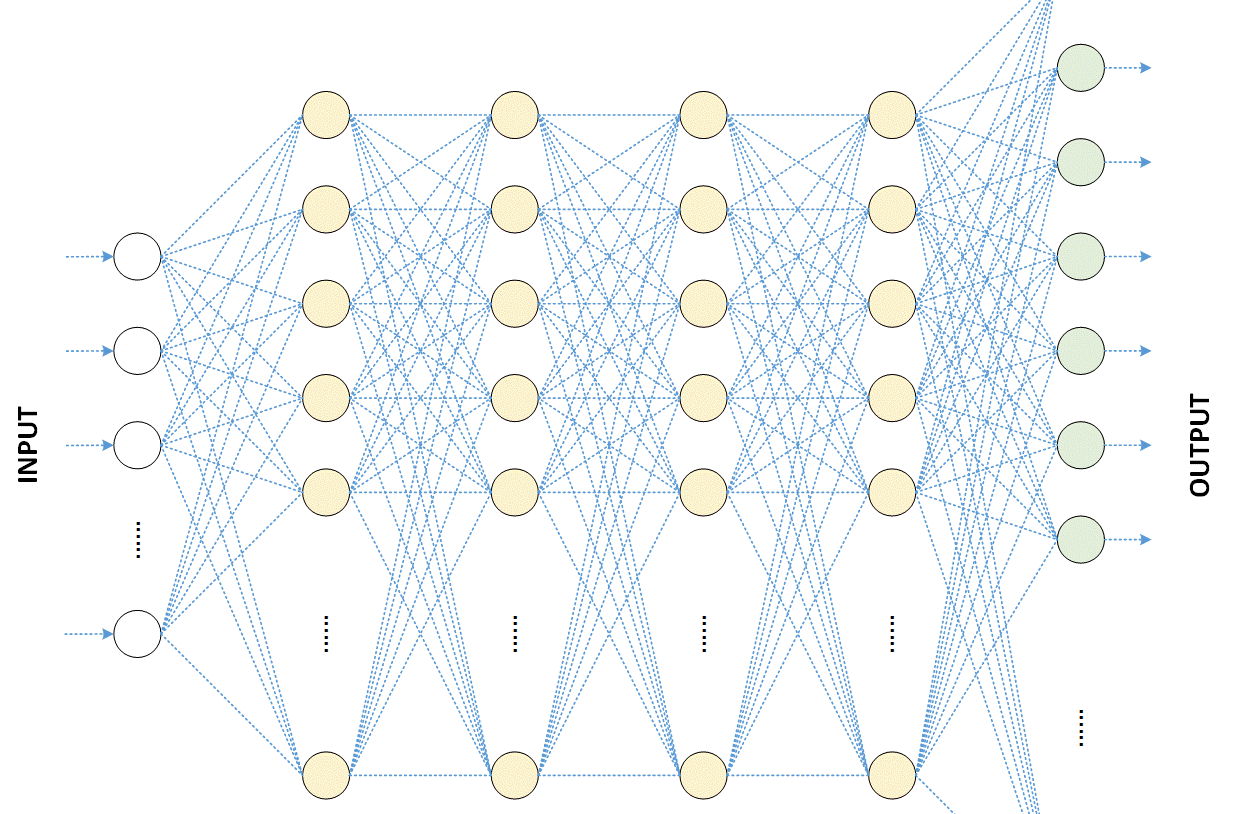
\includegraphics[width=0.65\linewidth]{network_dnn}
	\caption[]{\label{fig:network_dnn}
	DNN网络模型
	}
\end{figure}

\paragraph{深度学习框架}\cite{ wiki:Deep_learning}至今已有数种深度学习框架。包括深度神经网络、卷积神经网络和深度置信网络和递归神经网络。深度学习在计算机视觉、自然语言处理等方面已经取得了极好的效果。本文涉及的问题属于计算机视觉领域,深度学习的优越性正是选择的初衷。

深度神经网络是一种具备至少一个隐层的神经网络。深度神经网络具有更多网络层,如\cref{fig:network_dnn}示例,一般来说第一层是输入层,中间的层数为隐藏层,最后一层是输出层。

\paragraph{递归神经网络}\cite{ wiki:RNN}(Recurrent Neural Network,RNN)是一种节点定向连接成环的人工神经网络,属于深度学习网络的一种。
\begin{itemize}
  \item \textbf{编码器}递归神经网络将输入序列$\vec{x}$编码为一个固定长度的隐藏状态$\vec{h}$(以自然语言处理为例)
  \begin{itemize}
    \item $\vec{x}=\left(x_{t}, \ldots, x_{1}\right)$是输入序列。
    \item $\overrightarrow{h_{t}}=f\left(x_{t}, \overrightarrow{h_{t-1}}\right)$ 是随时间更新的隐藏状态。之前的状态$\overrightarrow{h_{t-1}}$转换为和当前输入$x_t$相关的$\overrightarrow{h_{t}}$。
  \end{itemize}
  其中,计算隐藏状态的方程$f(x,h)$是一个非线性方程,可以是复杂的\textbf{LSTM}单元(Long-ShortTerm Memory)。获得隐藏状态序列后,做出下一步预测:
  \begin{itemize}
    \item $p\left(y_{t}\right)=p\left(y_{t} | y_{t-1}, \ldots, y_{1}\right)$,其中$y_{t}$是第$t$个位置上的输出。
    \item 以上概率可以通过隐藏状态来计算:$p\left(y_{t}\right)=g\left(y_{t-1}, \overrightarrow{h_{t}}, \vec{c}\right), \vec{c}$是所有隐藏状态的编码,总含了所有隐藏状态。因为隐藏状态$t$就编码了第$t$个输入前全部的输入信息,$y_{t}$也迭代式地隐含了之前的全部输出信息。
  \end{itemize}
  \item \textbf{解码器}神经网络可以添加编码器作为解码器($Decoder$)。编码后($Encoded$)的信息通过解码器翻译为人类熟悉的信息。也就是上述例子中的$y_{t}=f\left(y_{t-1}, h_{t}, c\right)$过程,当中非线性模型$f$就是作为输出的复发神经网络。同时需要对$h_t^{'}$继续进行迭代:
  \begin{itemize}
    \item $h_{t}^{\prime}=g\left(h_{t-1}, y_{t-1}, c\right), \vec{c}$是解码器传递给编码器的参数,是解码器中状态的summary。$h_t^{'}$是解码器的隐藏状态。$y_t$是第$t$个输出。
    \item 当输入仍为$\vec{x}=\left(x_{t}, \ldots, x_{1}\right)$,输出是$\vec{y}=\left(y_{t}, \ldots, y_{1}\right)$,最大化条件概率$P(\vec{y} | \vec{x})$就是最好的结果。
  \end{itemize}
\end{itemize}

% \begin{figure}
% \centering
% \subfigure[RNN(左侧)和LSTM(右侧)对比] {
% \label{fig:lstm_rnn}
% 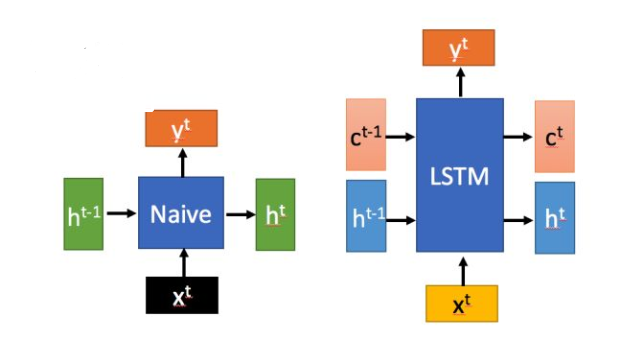
\includegraphics[width=0.65\textwidth]{lstm_rnn}
% }
% \subfigure[LSTM状态] {
% \label{fig:lstm_state}
% 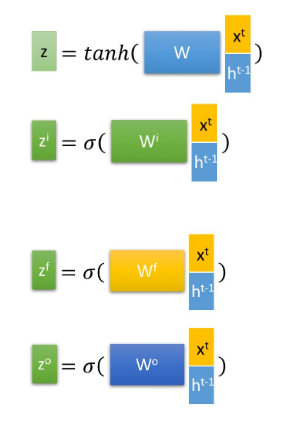
\includegraphics[width=0.3\textwidth]{lstm_fourstate}
% }
% \subfigure[LSTM内部结构] {
% \label{fig:lstm_inside}
% 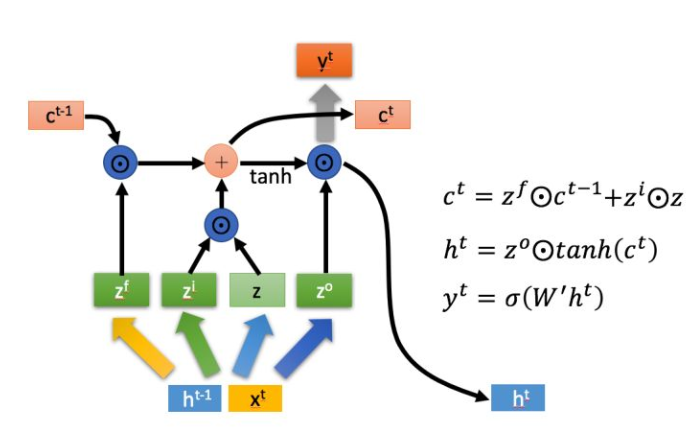
\includegraphics[width=\textwidth]{lstm_inside}
% }
% \end{figure}

\paragraph{长短期记忆}\cite{ wiki:LSTM}($Long short-term memory$, LSTM)是人工递归神经网络(RNN)的一种模式,广泛地运用于深度学习领域。与标准的前馈神经网络不同,LSTM具有反馈机制。LSTM不仅可以处理单个数据点,也可以处理整个数据序列。

一个通用的LSTM单元由单元,输入门,输出门和遗忘门组成。单元负责记住任意时间间隔内的值。三个门控制进出单元的信息流。

LSTM非常适合于对时间序列数据的分类任务、处理任务等。因为在时间序列中,重要事件之间可能存在未知的滞后和联系。LSTM提出的初衷就是为了处理在训练传统RNN时可能遇到的梯度爆炸和梯度消失问题。LSTM的优势还在于该网络对于间隙长度的不敏感性。

\begin{itemize}
  \item LSTM架构有很多种。常见的LSTM架构由单元(LSTM单元的存储器部分)和LSTM单元内部信息流的三个“调节器”组成:输入门,输出门和遗忘门。 一些变形的LSTM单元可能不具有一个或多个门,或者可能具有其他类型的门。单元负责跟踪输入序列中的元素之间的依赖性。输入门控制新值流入单元的程度,忘记门控制值在单元中保留的程度,输出门中的值用于计算输出的程度从而激活LSTM单元。 LSTM门的激活功能通常是逻辑功能。
  \item 具有遗忘门的LSTM单元的正向通过的形式如下:
  \begin{equation}
    \begin{aligned} f_{t} &=\sigma_{g}\left(W_{f} x_{t}+U_{f} h_{t-1}+b_{f}\right) \\ i_{t} &=\sigma_{g}\left(W_{i} x_{t}+U_{i} h_{t-1}+b_{i}\right) \\ o_{t} &=\sigma_{g}\left(W_{o} x_{t}+U_{o} h_{t-1}+b_{o}\right) \\ c_{t} &=f_{t} \circ c_{t-1}+i_{t} \circ \sigma_{c}\left(W_{c} x_{t}+U_{c} h_{t-1}+b_{c}\right) \\ h_{t} &=o_{t} \circ \sigma_{h}\left(c_{t}\right) \end{aligned}
  \end{equation}其中初始值为$c_ {0} = 0$且$h_ {0} = 0$和运算符$\circ$表示$Hadamard$。下标$t$为时间步长。
  式子中变量定义如下:
  \begin{itemize}
    \item $x_{t} \in \mathbb{R}^{d}$:LSTM单元的输入向量。
    \item $f_{t} \in \mathbb{R}^{h}$:遗忘门的激活向量。
    \item $i_{t} \in \mathbb{R}^{h}$:输入门的激活向量。
    \item $o_{t} \in \mathbb{R}^{h}$:输出门的激活向量。
    \item $h_{t} \in \mathbb{R}^{h}$:隐藏状态向量,也称为LSTM单元的输出向量。
    \item $c_{t} \in \mathbb{R}^{h}$:单元状态向量。
    \item $W \in \mathbb{R}^{h \times d}, U \in \mathbb{R}^{h \times h}$ 和 $b \in \mathbb{R}^{h}$:权重矩阵和偏差参数。
  \end{itemize}
  式子中的激活函数如下:
  \begin{itemize}
    \item $\sigma_{g}$:$sigmoid$ 函数。
    \item $\sigma_{c}$:双曲正切函数。
    \item $\sigma_{h}$:双曲正切函数。
  \end{itemize}
\end{itemize}

% !TeX root = ../Main/XMU.tex
\chapter{方法}{Methodology}
在本节中,将会完整阐述本文提出的基于监督学习方法的IK解算器。

\cref{fig:flowchart}说明了我们方法的整体流程。 CMU的动作捕捉库中的BVH文件是训练集和测试集的来源。在MATLAB中,对BVH文件进行解析和整合后,提取出神经网络的训练集和测试集。训练集和测试集一共三组,分别对应$\mathbf{MP}$和$\mathbf{PE}$和去噪滤波器(具体定义见\ref{sec:components}),六个文件,总大小超过$10$GB。$\mathbf{MP}$和$\mathbf{PE}$训练后,通过预先训练好的去噪滤波器,进一步对预测的姿态进行修正,得到最终结果。具体应用$\mathbf{IK}$解算器时,输入的轨迹(向量序列)依次经过$\mathbf{MP}$和$\mathbf{PE}$和去噪滤波器,得到最终的预测姿态。

本文方法的关键组件是Motion Predictor(MP)和Posture Estimator(PE)。前者根据当前运动轨迹来预测末端效应器的未来位置,而后者基于一系列末端效应器位置估计身体姿势。同时加入了去噪滤波器对网络的原始输出姿态进行修正,在很大程度上使预测的姿态更自然、更流畅。
\begin{figure}[!h]
	\centering
	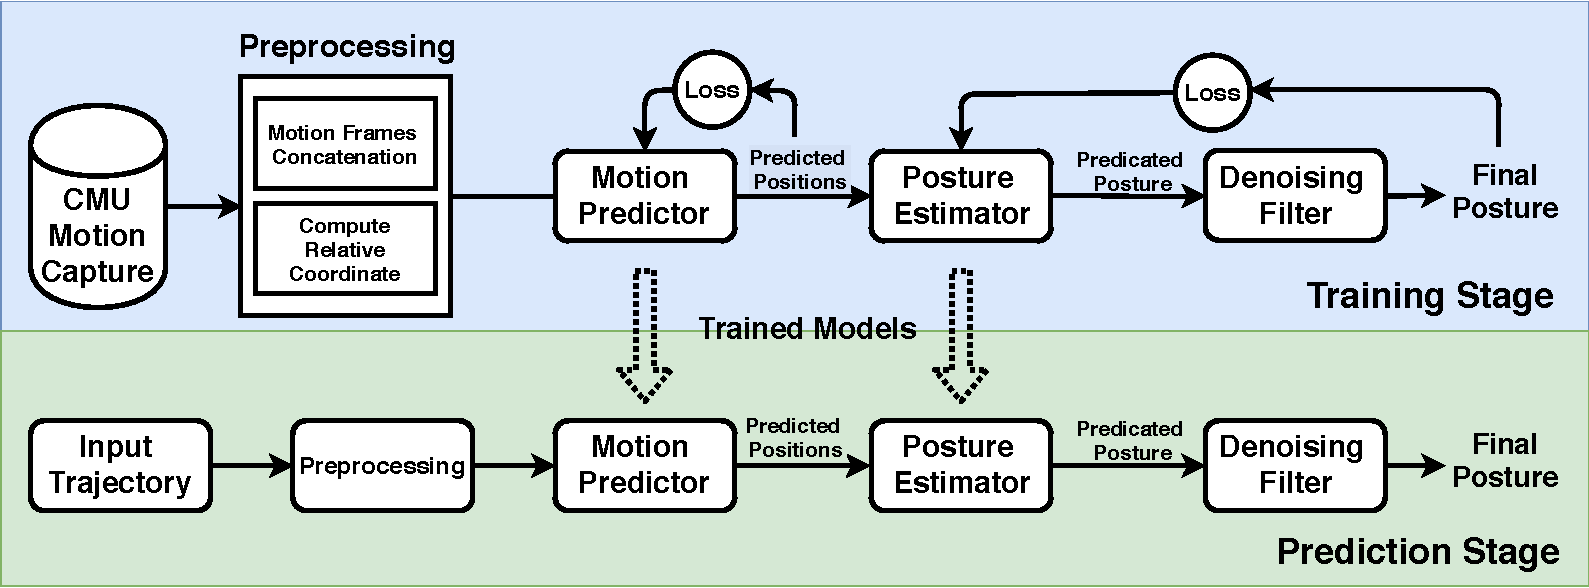
\includegraphics[width=\linewidth]{flowchart}
	\caption[]{\label{fig:flowchart}
		本方法的流程图
	}
\end{figure}

首先对本文中使用的一些术语进行定义:
\begin{itemize}
	\label{item:identify}
\item\textbf{骨骼(skelton)}骨骼$\mathbf{S}$定义具有根关节及其相互连接的关节角色的层次结构,而关节距离适用于构造具有几何变量的角色。
\item\textbf{末端执行器(end-effector)}末端执行器$\mathbf{EE}$通常指与环境进行交互的角色的脚和手。
\item\textbf{姿态(posture)}姿态$\mathbf{P}$是描述角色身体结构的向量,由根关节的全局变换和关节方向的角度值组成。
\item\textbf{动作(motion)}动作$\mathbf{M}$是一个矩阵,用于描述时域中的一系列角色姿势。矩阵行数对应帧数,列数与关节通道数成比例。
\item\textbf{位置(position)}位置$\mathbf{PE}$描述$\mathbf{EE}$的全局位置。
\end{itemize}

\section{离线网络学习}{Offline Network Learning}
\subsection{数据集和预处理}{Datasets and Preprocessing}
本次毕业论文使用Carnegie Mellon University(CMU)的Mocap数据库来构建此问题中的神经网络的训练集和测试集。 训练数据集包含约2000个动作序列(约200万个骨骼姿势),而测试数据集包含约200个动作序列(约20万个骨骼姿势)。运用MATLAB构建训练集和测试集时,使用正向运动学技术来计算骨骼关节的世界坐标位置。 我们提出了一种分层结构,将人体的四肢假设为互相独立的。所以整个人体姿态预测可以由四个独立的IK解算器组成,分别用于计算左/右臂和左/右腿。

我们定义了两种有效的技巧用来提高神经网络的学习性能:

\textbf{建立连续帧之间的时间关联性}过往的实验中,在解决\textbf{IK}问题时,往往只是将其归类为一个复杂的数学问题,忽视了它也是一个运动学问题,具备一定的时间关联性。实验证明,将连续的多帧的运动序列$[\cdots, X_{t-2*k}, X_{t-k},$ $ X_{t}, X_{t+k}, X_{t+2*k},\cdots]$替代传统的以末端执行器的当前位置作为网络输入在提高预测精度方面是有效的。 这在我们的实验中得到了证实(见\cref{fig:comparison_num_inputs}和章节\ref{sec:different_nums})。

\textbf{运用肩关节-腕关节/髋关节-踝节的相对坐标}在本次毕业论文中,通过计算肩关节-腕关节和髋关节-踝关节的相对向量来表示手臂和腿部的末端效应器的当前位置。采取这样的近似处理基于以下假设:股骨:胫骨和肱骨:尺骨的比例在个体之间的差异非常小。越来越多的研究表明,人虽然在身高和体重上的差别巨大,但是骨骼的比例确相差不多。而这样的处理也允许训练完毕后的IK解算器能够适应具有不同几何长度和几何形状的的角色,即无需得到待解决角色的肢体长度,也能预测出符合自然动作和流畅的姿态序列,这在以往的研究中是不存在的。

通过这些技巧,我们可以构建神经网络监督学习中\*X和\*Y之间的映射:

\begin{itemize}
\item $\mathbf{X}$:向量$N_X$表示从分层骨骼结构和动作联合通道中帧序列中末端效应器的全局位置。
\item $\mathbf{Y}$:向量$N_Y$表示身体各个关节方向的旋转角度值(BVH文件中角度的定义为欧拉角)。训练集和测试集中的该值直接从动作文件的相应通道进行复制。后续的操作中,为了提高神经网络的训练过程的表现,防止深层神经网络出现梯度爆炸、梯度消失等情况,对该值做了数学方法的处理(标准化),但不改变该值的原始定义和所表达的意义。
\end{itemize}

\subsection{IK解算器关键组件}{Main Components of IK Solver}
\label{sec:components}
Motion Predictor($\mathbf{MP}$)和Posture Estimator($\mathbf{PE}$)MP和PE是我们IK解算器的两个主要组成部分,我们使用大致相同的神经网络结构来构建这两个组件(需要指出,网络的输入输出是不同的)。 该网络的隐藏层是递归神经网络(RNN),具有三层LSTM(每层的大小为512),输入层和输出层是全连接层。

\begin{figure}[!h]
	\centering
	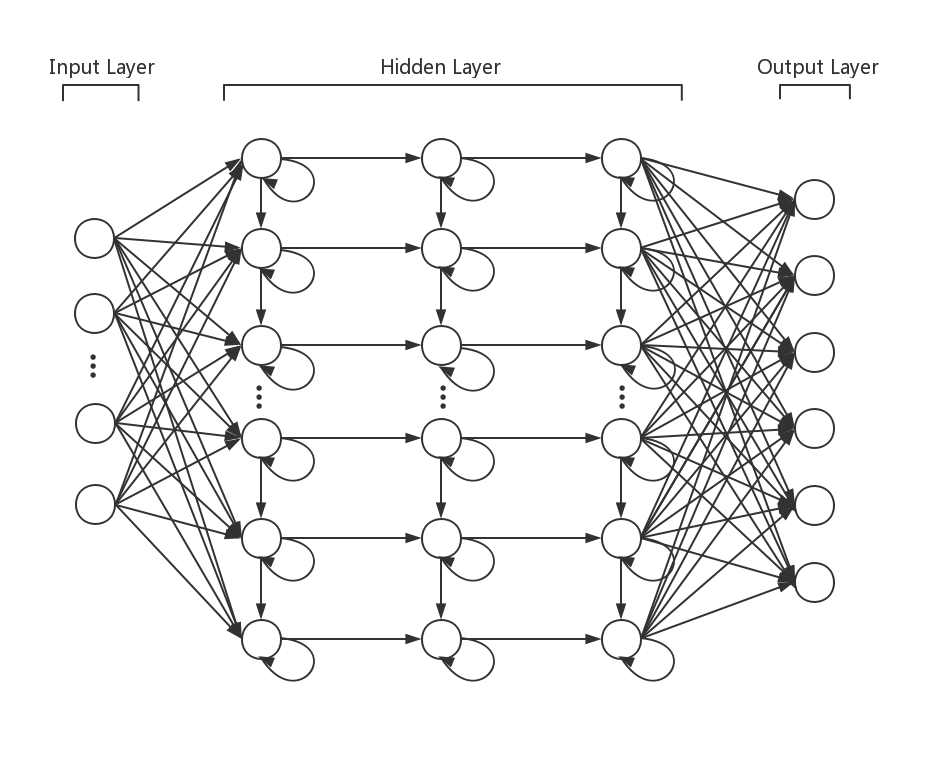
\includegraphics[width=0.8\linewidth]{network_mp}
	\caption[]{\label{fig:network_mp}
	$\mathbf{MP}$组件的网络结构
	}
\end{figure}
\paragraph{$\mathbf{MP}$网络结构}\cref{fig:network_mp}说明了$\mathbf{MP}$组件所用的神经网络的网络结构,该网络的输入是过去$\mathbf{K}$帧中的$\mathbf{EE}$位置序列,输出是下一个$\mathbf{K}$帧中的$\mathbf{EE}$位置序列。具体实现时,输入的帧数为$3$帧。设当前帧为第$i$帧,输入为第$i-10$帧、第$i-5$帧和第$i$帧。输入层有9个节点,分别表示输入帧各自的相对向量。输出的帧数为$2$帧。设当前帧为第$i$帧,输出为第$i+5$帧和第$i+10$帧。输出层共6个节点,分别表示输出帧各自的相对向量。将输入的帧数和输出的帧数进行整合后是$\mathbf{PE}$的输入。
\paragraph{$\mathbf{MP}$损失函数}

该神经网络的损失函数定义为:
\begin{equation}
L_m = \sum_{i=0}^{K_m} (\mathbf{PE}_i - \mathbf{PE}_i^G)
\end{equation}
该式中,$K_m$表示连续帧的帧数,$\mathbf{PE}_i^G$表示来自运动捕捉数据库的真实值.

\begin{figure}[!h]
	\centering
	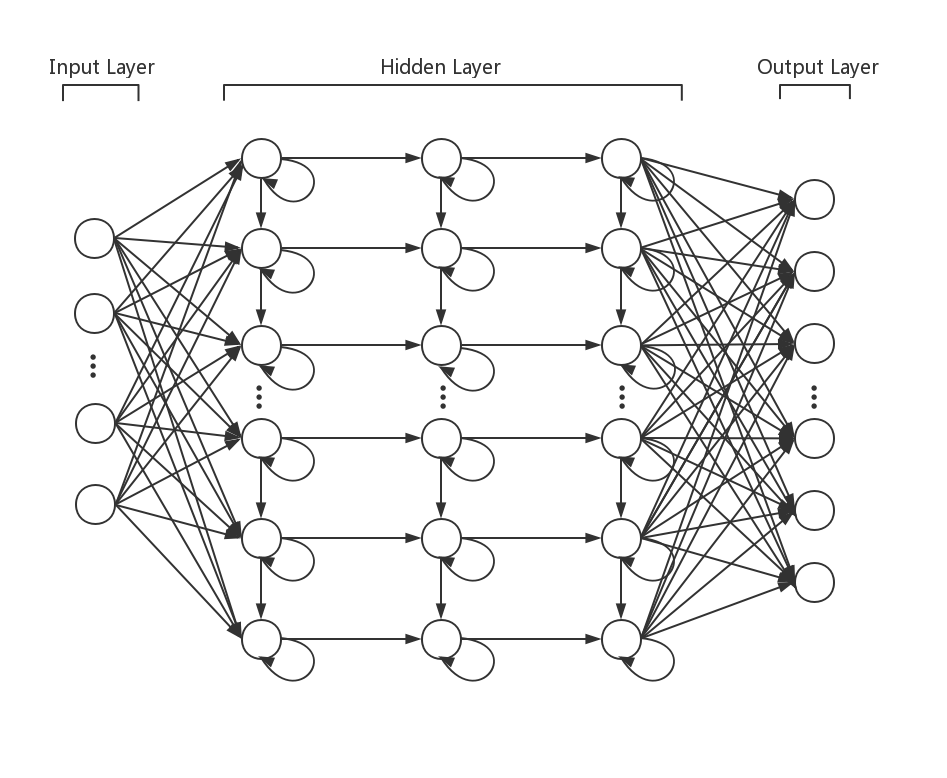
\includegraphics[width=0.8\linewidth]{network_pe}
	\caption[]{\label{fig:network_pe}
	$\mathbf{PE}$组件的网络结构
	}
\end{figure}

\paragraph{$\mathbf{PE}$网络结构}
\cref{fig:network_pe}说明了$\mathbf{PE}$组件所用的神经网络的网络结构,该网络的输入是过去$\mathbf{K}$帧中、当前帧和下一个$\mathbf{K}$帧中的位置序列,输出是过去当前帧和下一个$\mathbf{K}$帧中的$\mathbf{EE}$预测姿势序列。 具体实现时(以右手臂为例),输入的帧数为5帧。设当前帧为第$i$帧,输入的帧为第$i-10$帧、第$i-5$帧、第$i$帧和$\mathbf{MP}$输出的第$i+5$帧和第$i+10$帧,即将$\mathbf{MP}$
的输入和输出进行整合。输入层有15个节点,分别表示输入帧的各自相对向量。输出的帧数为$6$帧。设当前帧为第$i$帧,输出的帧为第$i$帧、第$i+1$帧、第$i+2$帧、第$i+3$帧、第$i+4$帧、第$i+5$帧。输出层有36个节点,,分别表示输出帧各自的肩关节和肘关节的旋转角。
\paragraph{$\mathbf{PE}$损失函数}
神经网络的损失函数定义为:
\begin{equation}
L_p = \sum_{i=0}^{K_p} (\mathbf{P}_i - \mathbf{P}_i^G)
\end{equation}
该式中,$K_p$表示连续帧的帧数,$\mathbf{P}_i^G$表示来自运动捕捉数据库的真实值。

\paragraph{激活函数、优化器和超参数}深度神经网络采用目前流行的RNN网络模型作为网络连接模式以适用连续帧之间的时间关联性,具体细节如下:
\begin{itemize}
	\item 选用线性整流函数(Rectified Linear Unit, ReLU)作为激活函数。线性整流函数定义了该神经元在线性变换$\mathbf{w}^{T} \mathbf{x}+b$之后的非线性输出结果。更加直观的理解为,对于来自上一层神经网络的输入向量$x$,该函数的神经元会输出$\max \left(0, \mathbf{w}^{T} \mathbf{x}+b\right)$。下一层神经元以此作为本层神经网络的输入。
	\item 选用Adam优化器作为优化函数。Adam结合AdaGrad和RMSProp两种优化算法的优点,对梯度的一阶矩估计(First Moment Estimation,即梯度的均值)和二阶矩估计(Second Moment Estimation,即梯度的未中心化的方差)进行综合考虑,计算出更新步长。更新规则如下:
	\begin{itemize}
		\item 计算时间梯度:$g_{t}=\nabla_{\theta} J\left(\theta_{\mathrm{t}-1}\right)$。
		\item 计算指数式的梯度移动的平均数,$\beta_1$为系数为指数衰减率,控制权重分配:$m_{t}=\beta_{1} m_{t-1}+\left(1-\beta_{1}\right) g_{t}$;$m_0$初始化为0。
		\item 计算梯度平方的指数移动平均数,$v_0$初始化为$0$。$\beta_2$系数为指数衰减率:$v_{t}=\beta_{2} v_{t-1}+\left(1-\beta_{2}\right) g_{t}^{2}$。
		\item 对梯度均值$m_t$进行偏差纠正,降低偏差对训练初期的影响:$\hat{m}_{t}=m_{t} /\left(1-\beta_{1}^{t}\right)$。
		\item 对$v_t$进行纠正:$\hat{v}_{t}=v_{t} /\left(1-\beta_{2}^{t}\right)$。
		\item 更新参数,初始的学习率$x$乘以梯度均值与梯度方差的平方根之比:$\theta_{\mathrm{t}}=\theta_{t-1}-\alpha^{*} \hat{m}_{t} /\left(\sqrt{\hat{v}_{t}}+\varepsilon\right)$。
	\end{itemize}
	\item 设置$batch size=128$,$learning_rate=0.0001$,$maximal epoch = 1000$。
\end{itemize}

\paragraph{网络参数调节}
在实际的训练过程中,为达到最好的训练效果,在模型的参数上和样本集的处理可能会做一些微调以达到更好的精度和更快的训练速度:
\begin{itemize}
\item{学习率自下降(learning rate adaptive decay)}防止学习率过大,在收敛到全局最优点的时候会来回摆荡,所以学习率随着训练轮数不断按指数级下降,收敛梯度下降的学习步长。

\item{梯度剪切(weithts regularization)}训练集的规模的约束导致了神经网络的层数在设计过程中需要比过往经验中的更多。正因如此,梯度爆炸和梯度消失的现象有可能在网络模型的参数调整过程中出现。为了解决这一问题,设计一个梯度阈值,如果超过该阈值,直接将梯度置为该值。
\end{itemize}

\subsection{去噪滤波器}{Denoising Filter}
\paragraph{平滑度}
合成动作的平滑度是IK技术成功与否的关键衡量标准之一\cite{aristidou2018inverse},特别是在一些涉及收敛的迭代算法中。通常,建议程序在固定的迭代次数之后终止循环以避免程序陷入无限循环。 然而,这个操作可能只能得到次优结果并导致合成动作的波动。
\paragraph{自然度}
评估一个动作序列是否是自然的是困难的因为它没有一个固定的标准,除此之外,这个标准可能根据不同的场景和主题而随之变化。本次毕业论文中,在自然度的评估是通过比较合成动作和原始动作数据之间的差异,差异越小则代表动作越自然。之所以能做出这样的标准是因为本文采用的动作数据来自真实的人体动作捕捉,并非通过计算机模拟产生。
\textbf{PE}网络的输出存在一定的噪音(连续帧之间动作不够平滑和自然,更直观的说法为视觉上骨骼轻微抖动)进一步使用平均滤波器进行处理以进行去噪。平均滤波器的处理过程如下:
\begin{equation}
	\label{equ:filter}
\mathbf{P} = \frac{1}{N} (\sum_i^{i+k} {\mathbf{P}_i}+\sum_{i-k}^i{\mathbf{P}_j})
\end{equation}
$\mathbf{P}_i$表示\textbf{PE}网络输出的连续预测姿势序列,$\mathbf{P_j}$表示由内存中读取的过往姿势序列。

具体实现中,设当前帧为第$x$帧,\ref{equ:filter}中$i=x-5$,$k=x+5$。从第$x-5$帧至第$x-1$帧为已知,因为是过往姿势序列,可以从内存中直接读取;从第$x$帧到第$x+5$帧为$\mathbf{PE}$网络的输出。最终得到的$\mathbf{P}$为降噪后的姿势形态。
\label{sec:denoising}
这一步显著提高了\textbf{PE}输出预测姿势序列的平滑度,具体降噪效果见\ref{res:denoising}。

\section{姿势合成和姿势估计}{Posture Synthesis and Estimation}

本次毕业论文的IK求解器应用于两个应用:姿势合成和姿态估计。

\subsection{姿势合成}{Posture Synthesis}在用户指定末端执行器的轨迹后,即末端执行器在三维世界坐标内的位置序列,以0.5秒的均匀间隔对轨迹进行采样,然后运用$\mathbf{IK}$解算器自动生成全身姿势。轨迹的生成由两个步骤组成:相对坐标的计算和运动帧级联。相对坐标的计算指的是(以右手臂为例):捕捉右臂的肩关节、肘关节、腕关节的末端执行器的位置,以~\ref{sec:Retargetting}中所示方法计算出某一个时刻某一个姿势唯一的右臂向量;运动帧级联指的是在构造输入数据时,加入本文提出的连续帧之间的时间关联性,整合出符合训练好的解算器组件输入格式的数据。预测程序的流程如\cref{fig:flowchart}所示。
\begin{figure}[!h]
	\centering
	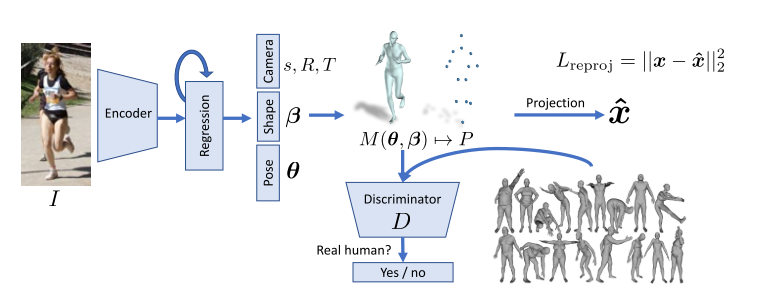
\includegraphics[width=\linewidth]{2dto3d}
	\caption[]{\label{fig:2dto3d}
	2D图像到3D人体骨骼预测流程\cite{kanazawa2018end}。输入的2D图像$I$首先通过$\mathbf{Encoder}$。$\mathbf{Encoder}$输出的结果传送到迭代$\mathbf{3D regression}$模块(该模块能够推断人的隐式三维表达方式来减少人体关节投影的误差)。3D参数也被发送到$\mathbf{Discriminator}$,鉴别器($\mathbf{Discriminator}$)$\mathbf{D}$的目的是告知这些参数是否来自真实的人体形状和姿势。
	}
\end{figure}
\subsection{姿态估计}{Posture Estimation}
本次毕业论文着重于改进使用单目摄像机捕捉图像到3D人体骨骼姿态的估计结果\cite{kanazawa2018end}。由于这是一个典型的不适定问题,所以解决该问题时具有一定的挑战性。

2D图像到3D人体骨骼的预测大致框架如\cref{fig:2dto3d}所示。涉及论文中提出直接利用以人为中心的单张RGB图像来重建人体完整的三维网格模型。神经网络训练过程中,假设所有图像都使用真实的二维关节进行注释,该方法还考虑了一些具有三维注释的情况。

除此之外,该方法假设有一个具有不同形状和姿势的人体三维网格池。由于这些网格不一定有相应的图像与之对应,因此我们将此数据称为未配对数据。\cref{fig:2dto3d}展示了所提出的预测网络架构。该网络可以执行端到端的训练。为了推断3D人体网格和相机,一张图像的卷积特征被发送到迭代3D回归模块,使得其3D关节投射到带注释的2D关节上。预测的人体参数传送到一个鉴别器网络。鉴别器的任务是确定3D参数是否是来自未配对数据。这步操作可以促进网络输出基于多样式人体形态的3D人体网格,并且能够作为没有真实3D注释的原始图像的弱监督。得益于3$L=\lambda\left(L_{\text { reproj }}+\mathbb{1} L_{3 \mathrm{D}}\right)+L_{\mathrm{adv}}$D网格模型具有多种表达方式,数据驱动先验方法可以捕获关节角度限制,人体测量约束(例如身高,体重,骨骼比率)。当拥有真实3D信息时,将其作为中间损失。总的来说,该方法的目标
\begin{equation}
	L=\lambda\left(L_{\text { reproj }}+\mathbb{1} L_{3 \mathrm{D}}\right)+L_{\mathrm{adv}}
\end{equation}其中$\lambada$控制每个物体的关联性的重要程度;$\mathbf{1}$是指示器函数,如果拥有真实值可用于图像则为1,否则为0。每个组件的具体实现如下:
\begin{itemize}
	\item \textbf{3D人体表达方式}该方法使用$\mathbf{SMPL}$模型来编码人体的3D网格
。形状参数$\boldsymbol{\beta} \in \mathbb{R}^{10}$由$\mathbf{PCA}$形状空间的前10个系数参数化得到。姿势参数$\boldsymbol{\theta} \in \mathbb{R}^{3 K}$$K = 23$个关节的相对3D旋转角来建模。 $\mathbf{SMPL}$是一个可微函数,它输出一个有$N=6980 $个顶点和
 $M(\boldsymbol{\theta}, \boldsymbol{\beta}) \in \mathbb{R}^{3 \times N}$ 的三角网格。通过线性回归得到的3D关键点($X(\boldsymbol{\theta}, \boldsymbol{\beta}) \in \mathbb{R}^{3 \times P}$)可以用于计算投影误差。
 \item \textbf{带回馈3D交互回归}3D回归模块的目标是输出带图像编码$\phi$的$\Theta$
使得联合重投影误差$L_{\text { reproj }}=\Sigma_{i}\left\|v_{i}\left(\mathbf{x}_{i}-\hat{\mathbf{x}}_{i}\right)\right\|_{1}$最小化。式中$\mathbf{x}_{i} \in \mathbb{R}^{2 \times K}$是第$i$个真实2D关节。$v_{i} \in\{0,1\}^{K}$是$K$个关节的各自是否可视化值。

3D回归模块将图像特征$\theta$和当前参数$\Theta_t$作为输入并输出残差$\Delta \Theta_{t}$。 通过将该残差加到当前估计$\Theta_{t+1}=\Theta_{t}+\Delta \Theta_{t}$来更新参数。 初始估计$\Theta_0$被设置为平均$\overline{\Theta}$。 以下是3D损失的定义:
\begin{equation}
\begin{aligned} L_{3 \mathrm{D}} &=L_{3 \mathrm{D} \text { joints }}+L_{3 \mathrm{D} \text { smpl }} \\ L_{\text { joints }} &=\left\|\left(\mathbf{X}_{\mathbf{i}}-\hat{\mathbf{X}}_{\mathbf{i}}\right)\right\|_{2}^{2} \\ L_{\text { smpl }} &=\left\|\left[\boldsymbol{\beta}_{i}, \boldsymbol{\theta}_{i}\right]-\left[\hat{\boldsymbol{\beta}}_{i}, \hat{\boldsymbol{\theta}}_{i}\right]\right\|_{2}^{2} \end{aligned}
\end{equation}
\item \textbf{分解对抗性先验}该工作使用经过训练的鉴别器网络$D$来判断$\mathbf{SMPL}$参数是否对应于人体真实值。将此称为对抗性先验,因为鉴别器充当引导3D预测的数据驱动先验。该方法镜像$\mathbf{SMPL}$的形状并进行了姿势分解,独立训练形状和姿势的鉴别器。因为姿势的预测基于动作树,所以进一步分解姿势鉴别器并单独为每个关节训练一个。为了捕获整个动作树的联合分布,训练一个接受所有旋转的鉴别器。由于每个鉴别器的输入是非常低的维度($\beta$为$10-D$,每个关节为$9-D$,所有关节为$9K-D$),因此训练的网络都可以是小型网络。所有姿势鉴别器共享旋转矩阵的共同特征空间,并且仅分别学习最终分类器。

在所有训练的$k+2$个鉴别器中,每个鉴别器$D_i$的输出介于$[0,1]$之间,用此来表示$\Theta$来自数据库的可能性。实际训练过程中,使用最小二乘法来保证其稳定性。设$E$表示包括图像编码器和3D模块的编码器。编码器的对抗性损失函数是:\begin{equation}
\min L_{\text { adv }}(E)=\sum \mathbb{E}_{\Theta \sim p_{E}}\left[\left(D_{i}(E(I))-1\right)^{2}\right]。
\end{equation}
每个鉴别器的目标是:\begin{equation}
\min L\left(D_{i}\right)=\mathbb{E}_{\Theta \sim p_{\text { data }}}\left[\left(D_{i}(\Theta)-1\right)^{2}\right]+\mathbb{E}_{\Theta \sim p_{E}}\left[D_{i}(E(I))^{2}\right]
\end{equation}
\end{itemize}


在实际的应用中,对于每个人体几何信息进行采集几乎是不可能的,所以本文所涉及的工作中,仅使用由2D图像到3D骨骼预测流程中输出的$\mathbf{EE}$的3D位置和与其对应的根关节位置,并应用本文提出的IK解算器对当前身体骨骼连接做出一个最佳姿态的估计。

% !TeX root = ../Main/XMU.tex
\chapter{实验结果和讨论}{Result and Discussions}
\section{实验细节}{Implementation Details}
\label{sec:implementation}
深度学习网络的训练环境和测试环境如下:
\begin{itemize}
	\item{操作系统:}Ubuntu 16.04
	\item{CPU:}Inter i7 7800k
	\item{GPU:}Nvidia Geforce TitanXP
	\item{内存:}16G
\end{itemize}
实验所需的材料(包括代码、训练集、测试集)发布在github上\footnote{link: https://github.com/uhomelee/DeepInverseKinematicsSolver}。整个训练过程需要大约36小时。
\begin{figure}[!htbp]
	\centering
	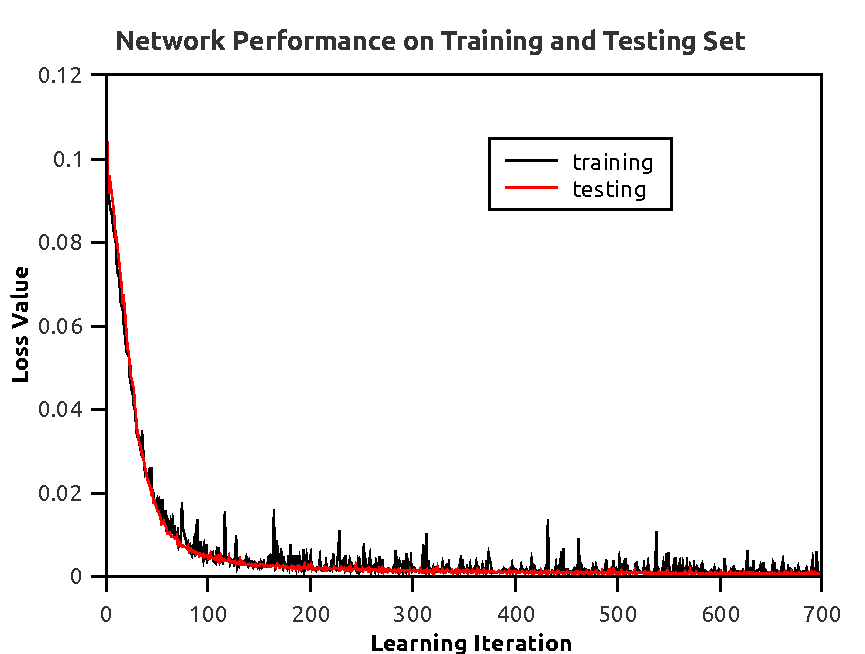
\includegraphics[width=0.75\linewidth]{loss_train_test}
	\caption[]{\label{fig:train_test}
		训练集和测试集比较
	}
\end{figure}
\begin{figure}
\centering
\subfigure[篮球运球动作] {
\label{fig:train_screenshot_dribble}
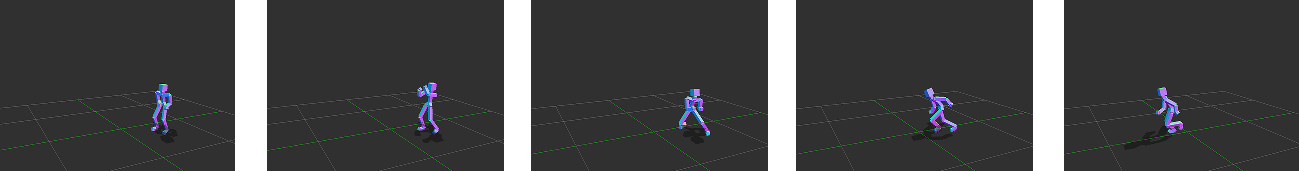
\includegraphics[width=\textwidth]{train_screenshot_dribble}
}
\subfigure[篮球投篮动作] {
\label{fig:train_screenshot_shooting}
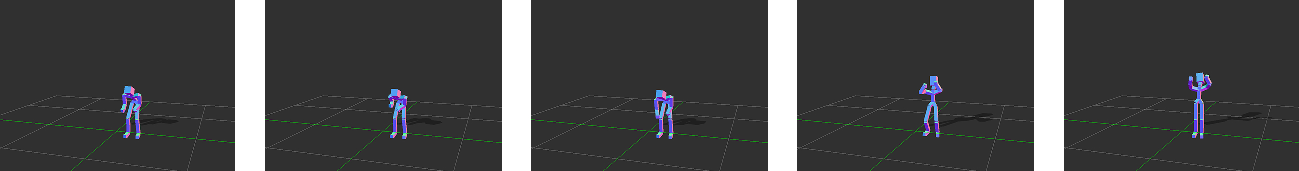
\includegraphics[width=\textwidth]{train_screenshot_shooting}
}
\subfigure[芭蕾舞动作] {
\label{fig:train_screenshot_dancing}
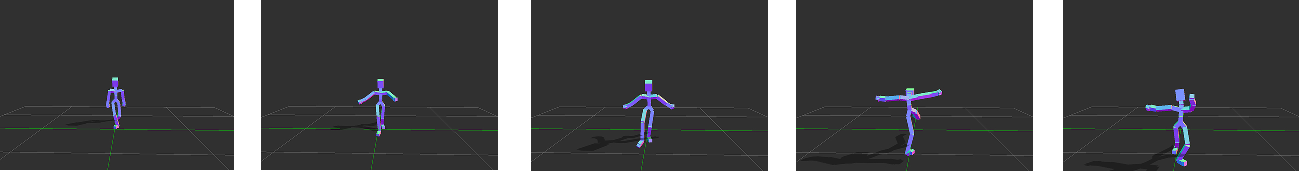
\includegraphics[width=\textwidth]{train_screenshot_dancing}
}
\caption{训练动作数据库合成动作}
\label{fig:train_screenshot}
\end{figure}
\begin{figure}
\centering
\subfigure[坐-起立动作] {
\label{fig:test_screenshot_gettingup}
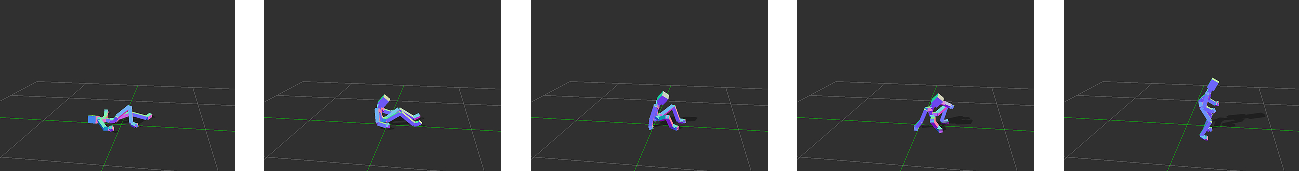
\includegraphics[width=\textwidth]{test_screenshot_gettingup}
}
\subfigure[篮球运球动作] {
\label{fig:test_screenshot_dribbling}
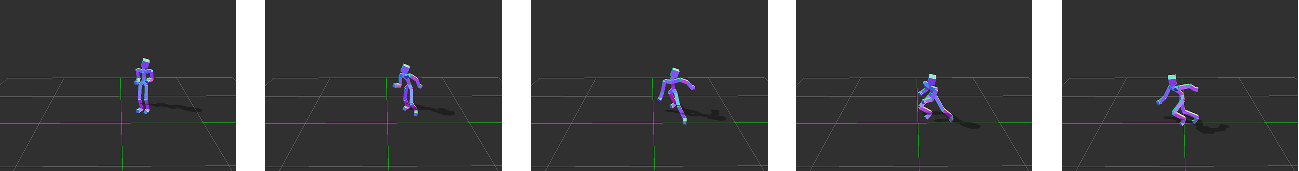
\includegraphics[width=\textwidth]{test_screenshot_dribbling}
}
\subfigure[翻跟头动作] {
\label{fig:test_screenshot_rolling}
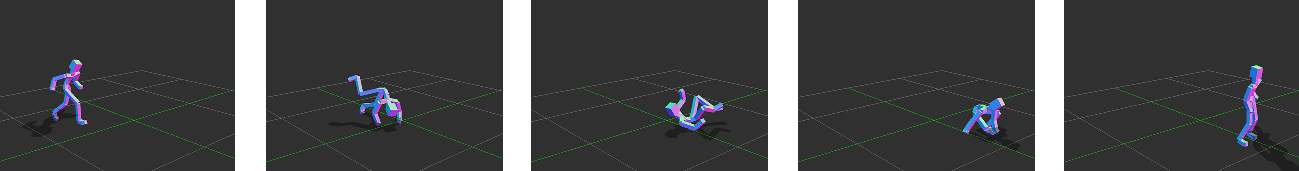
\includegraphics[width=\textwidth]{test_screenshot_rolling}
}
\caption{测试动作数据库合成动作}
\label{fig:test_screenshot}
\end{figure}
\section{实验结果}{Result}
\subsection{训练集和测试集结果}{Results on Training and Testing Dataset}
神经网络的训练集和测试集输出结果全部通过MATLAB脚本替代原有的BVH文件的数据值,并通过BVH PLAYER进行播放。训练结果可以通过两方面来检测,一是BVH文件的播放后的视觉效果,二是观察训练过程中训练集和测试集的损失函数值。


% \cref{fig:train_screenshot}展示了来自训练集的合成动作(包括篮球运球、投篮和芭蕾舞动作)。这些示例都需要角色对象进行精细的操作(例如对篮球的掌控)以及与环境频繁的交互(例如地面上的脚部支撑)。 这些动作的求解都需要ik解算器具备较高的精度。 一般来说,训练样本的最优的平均损失$<10^{-5}$,实际的预测的欧拉角和真实值的相差约在$\pm0.01^{\circe}$之间。

\cref{fig:test_screenshot}展示了来自测试集中的合成动作(包括从地面起立、篮球运球和翻跟斗)。
尽管这些例子中的动作并未包含在训练集中,但IK解算器仍可以解决该问题并产生符合自然姿态的动作。需要指出的是,测试集上的结果并未出现过拟合的情况,如\cref{fig:train_test}所示,训练集和测试集的损失函数值随着迭代次数的递增而下降,最终的结果测试样本的平均损失在$10^{-4}~10^{-5}$之间。通过实验,在全连接(FCN)模型中,虽然训练集上的网络性能表现良好,但在测试集上非常容易出现过拟合的情况。

\begin{figure}[!htbp]
	\centering
	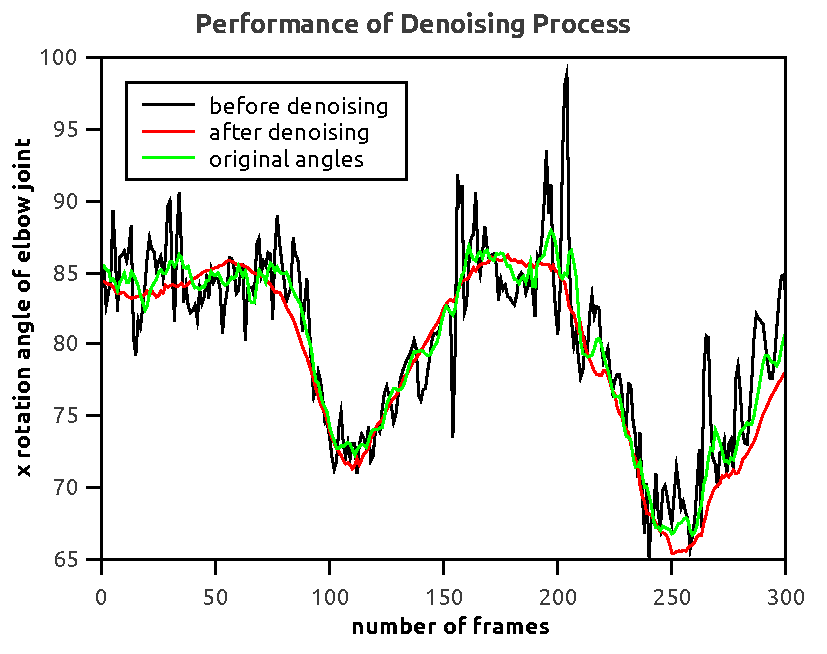
\includegraphics[width=0.75\linewidth]{denoising}
	\caption[]{\label{fig:denoising}
		去噪滤波器处理前后和真实值对比
	}
\end{figure}
\subsection{去噪滤波器结果}{Result on Denoising Filter}
尽管网络模型的损失函数在训练结束后收敛得非常小,但\textbf{IK}问题的求解的另一个需要考虑的因素是合成连贯动作后的自然度。考虑到$\mathbf{PE}$组件的输出在BVH PLAYER上播放时在某些复杂的动作(例如频繁的上下抬手、大范围的移动等情况)时出现的视觉上的抖动问题,对$\mathbf{PE}$组件的输出进行了降噪,具体的方法见\ref{sec:denoising}。如\cref{fig:denoising}所示,降噪的结果可以说是非常显著的。在BVH PLAYER上播放后,原先已经符合视觉上自然流畅的动作会显得更加自然(避免了太大角度的弯曲,违背了人体关节的旋转极限);原先有抖动的文件,在经过降噪后,基本可以做到流畅和自然。
\label{res:denoising}

\subsection{姿态估计结果}{Result on Posture Estimation}
\begin{figure}
\centering
\subfigure[] {
\label{fig:2dtobvh1}
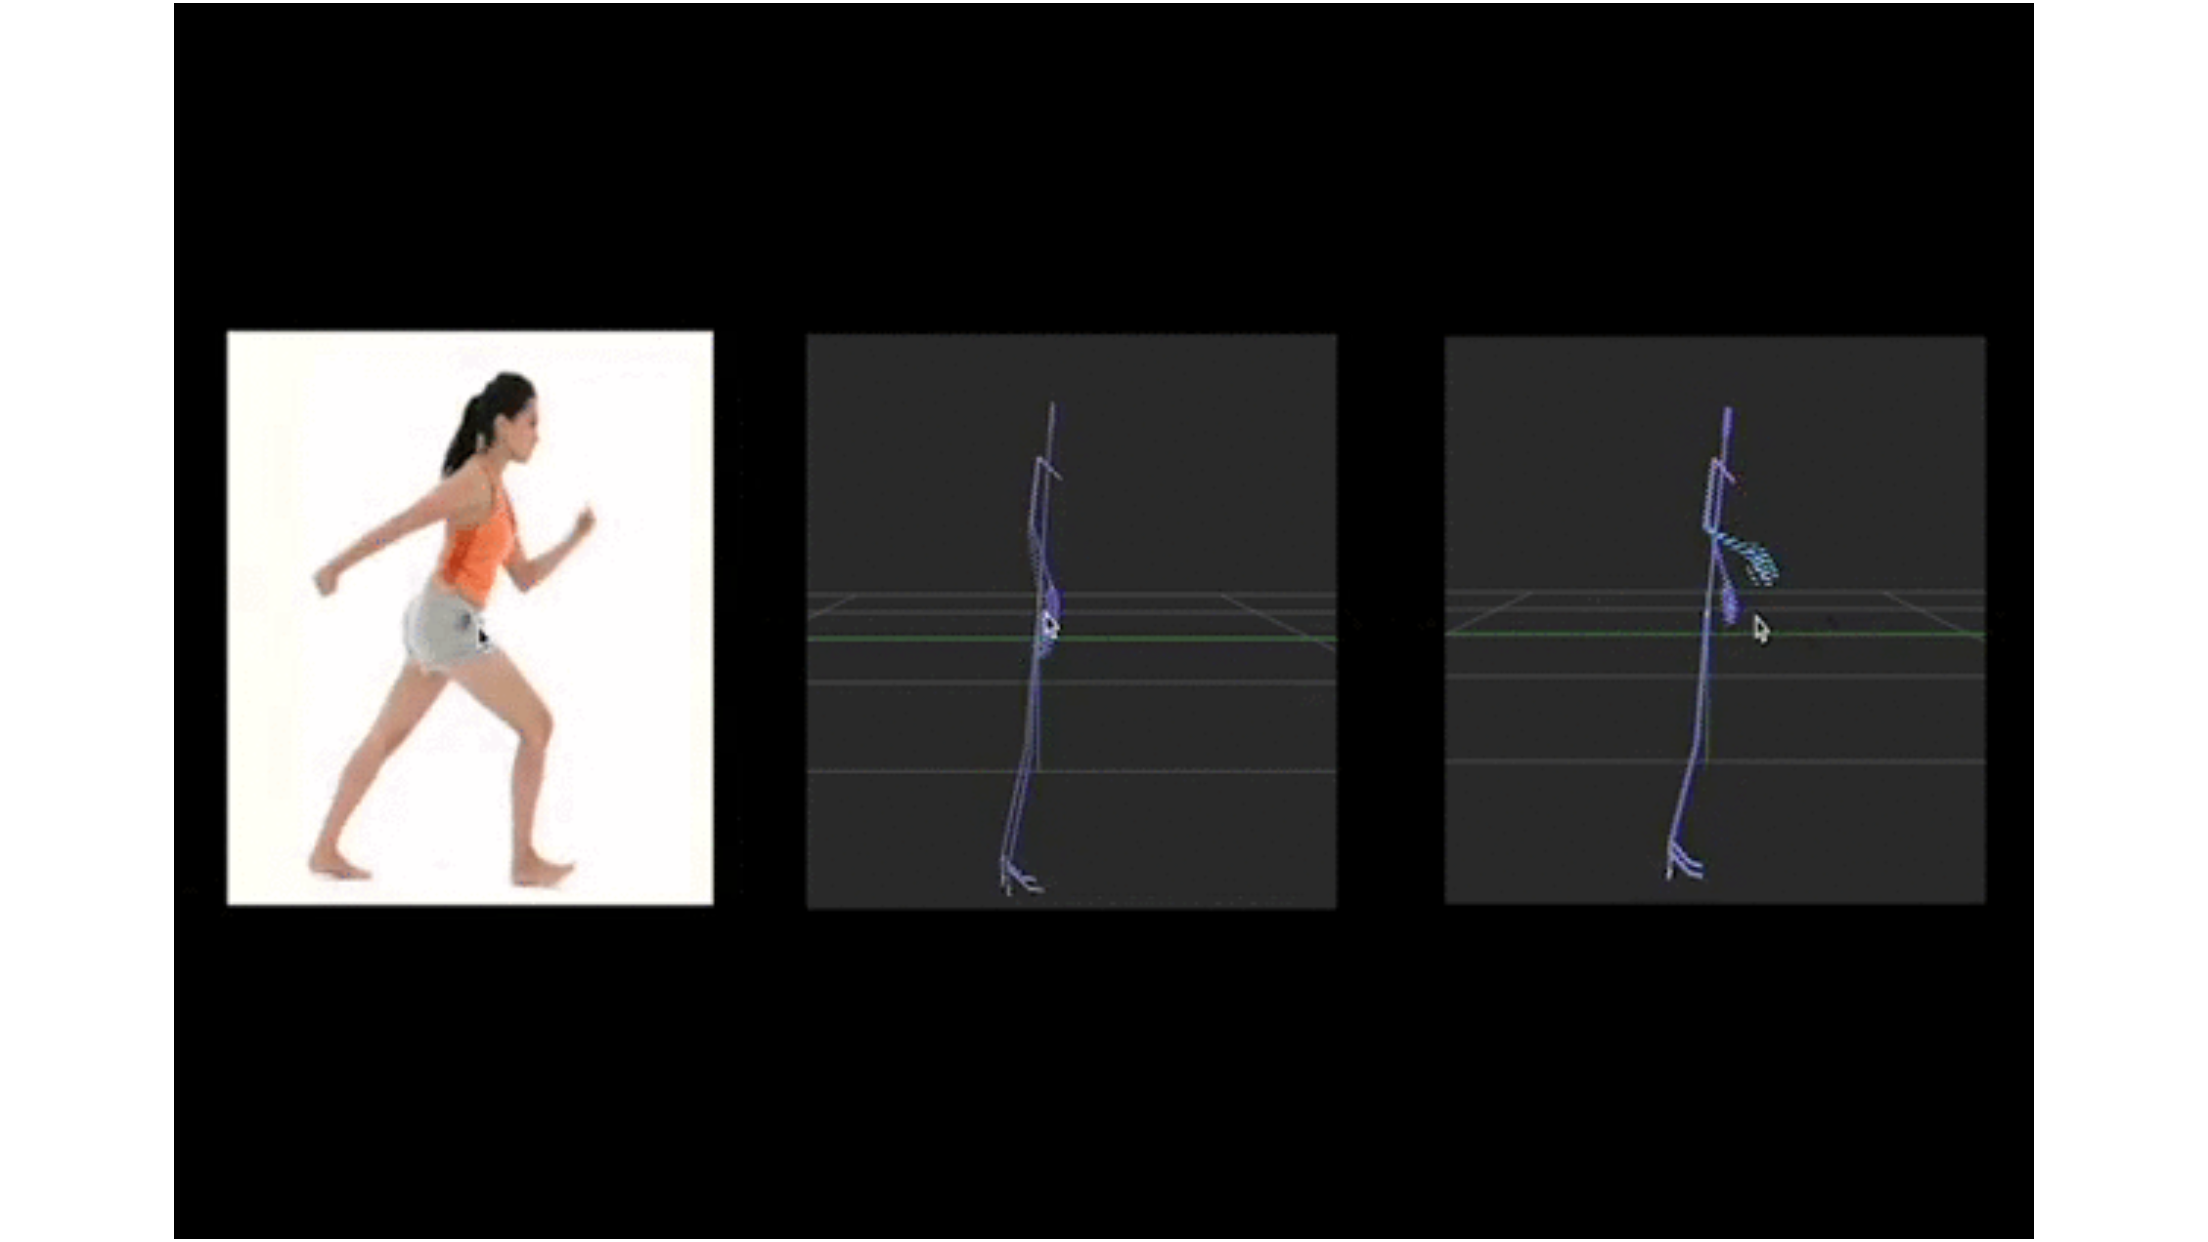
\includegraphics[width=0.3\textwidth]{2dtobvh1}
}
\subfigure[] {
\label{fig:2dtobvh2}
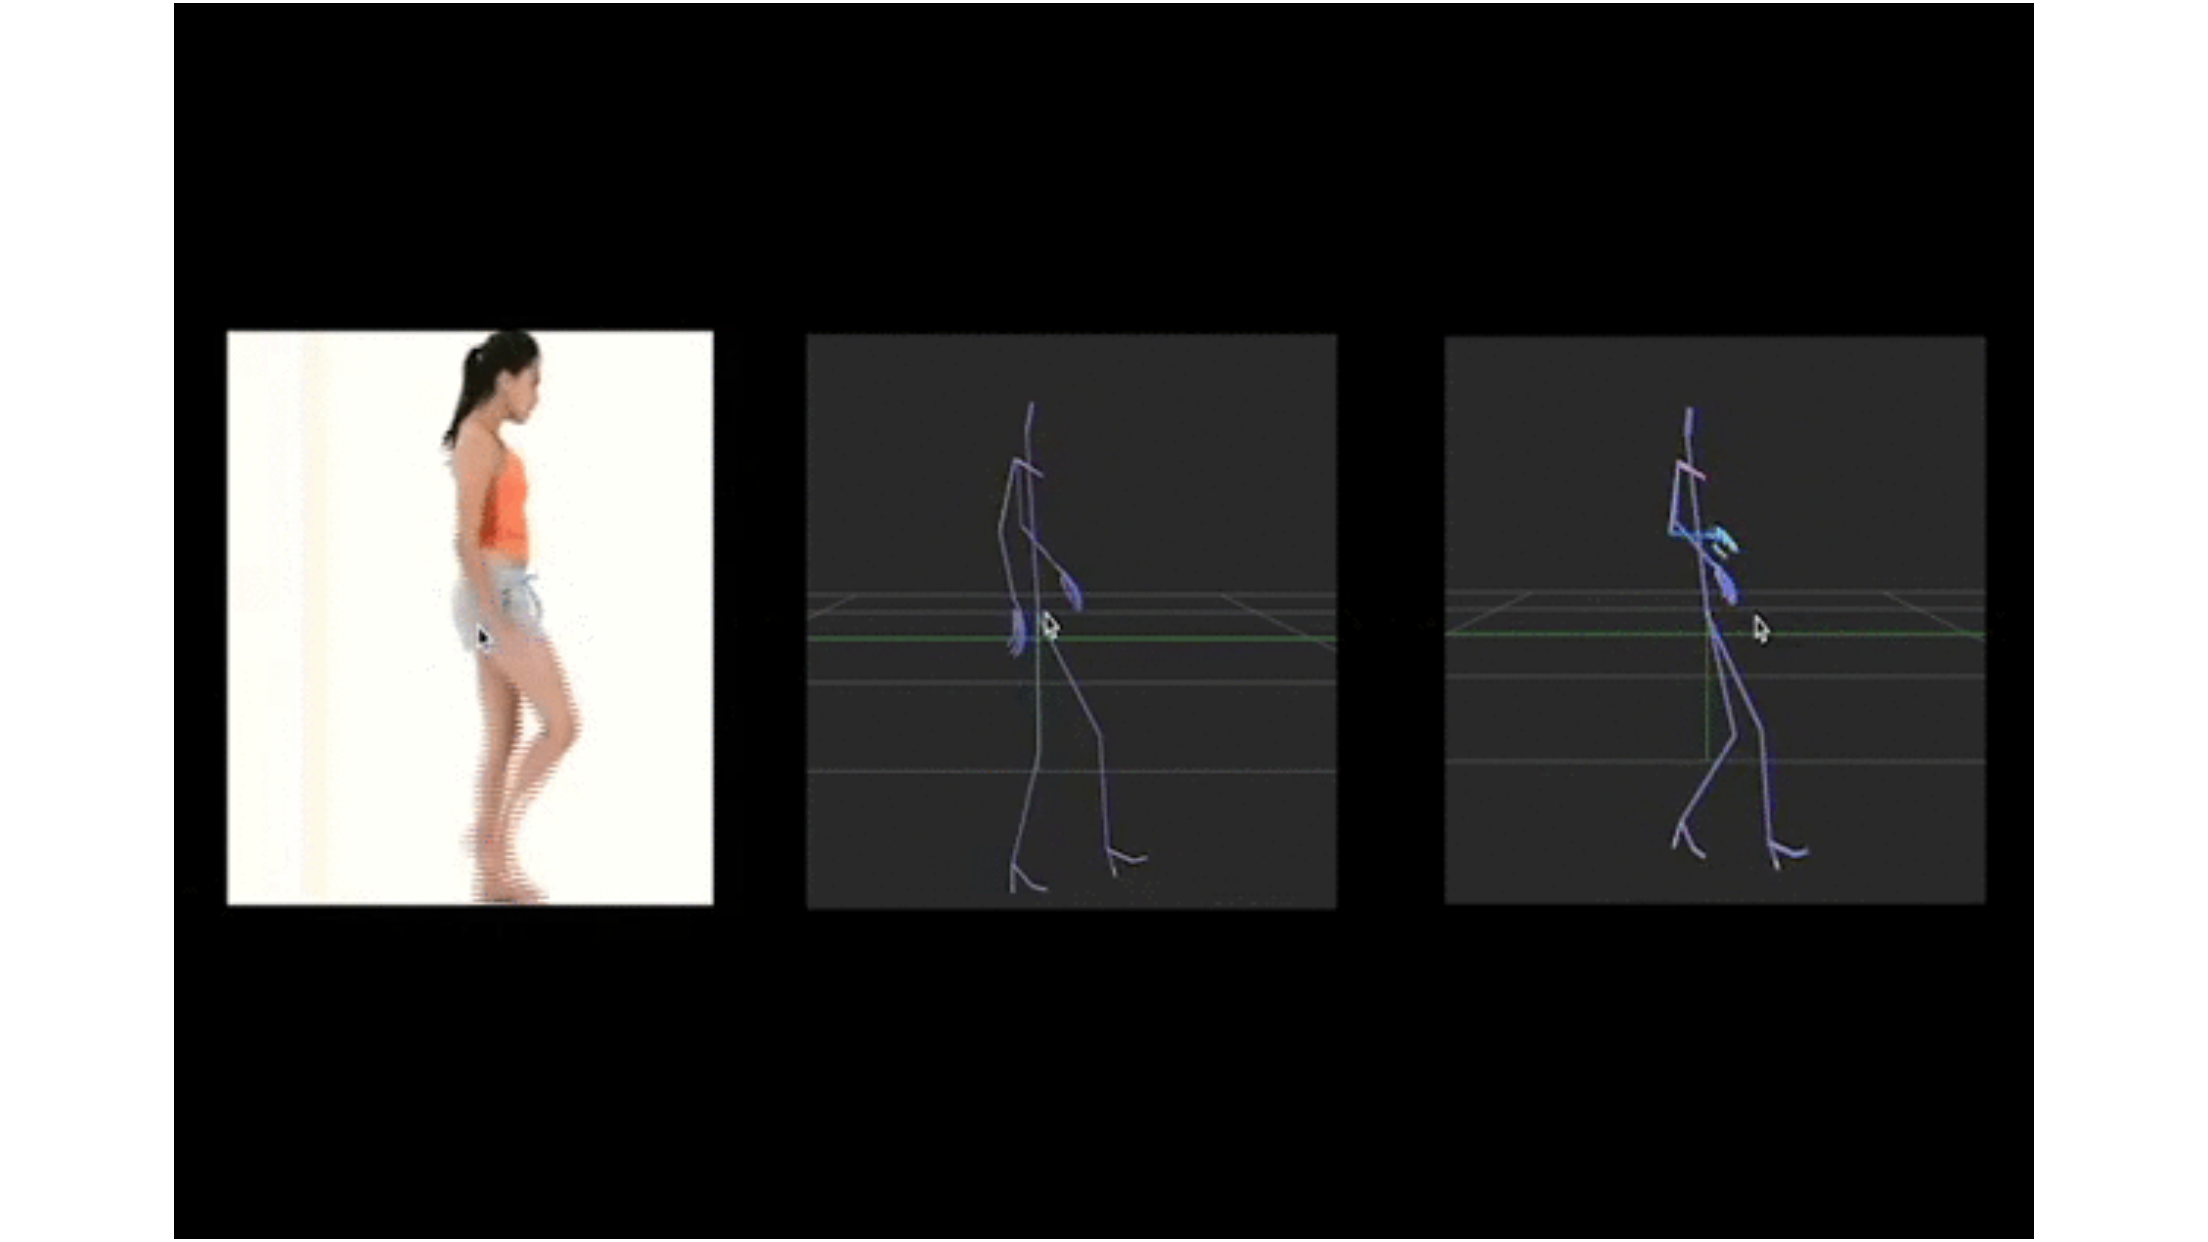
\includegraphics[width=0.3\textwidth]{2dtobvh2}
}
\subfigure[] {
\label{fig:2dtobvh3}
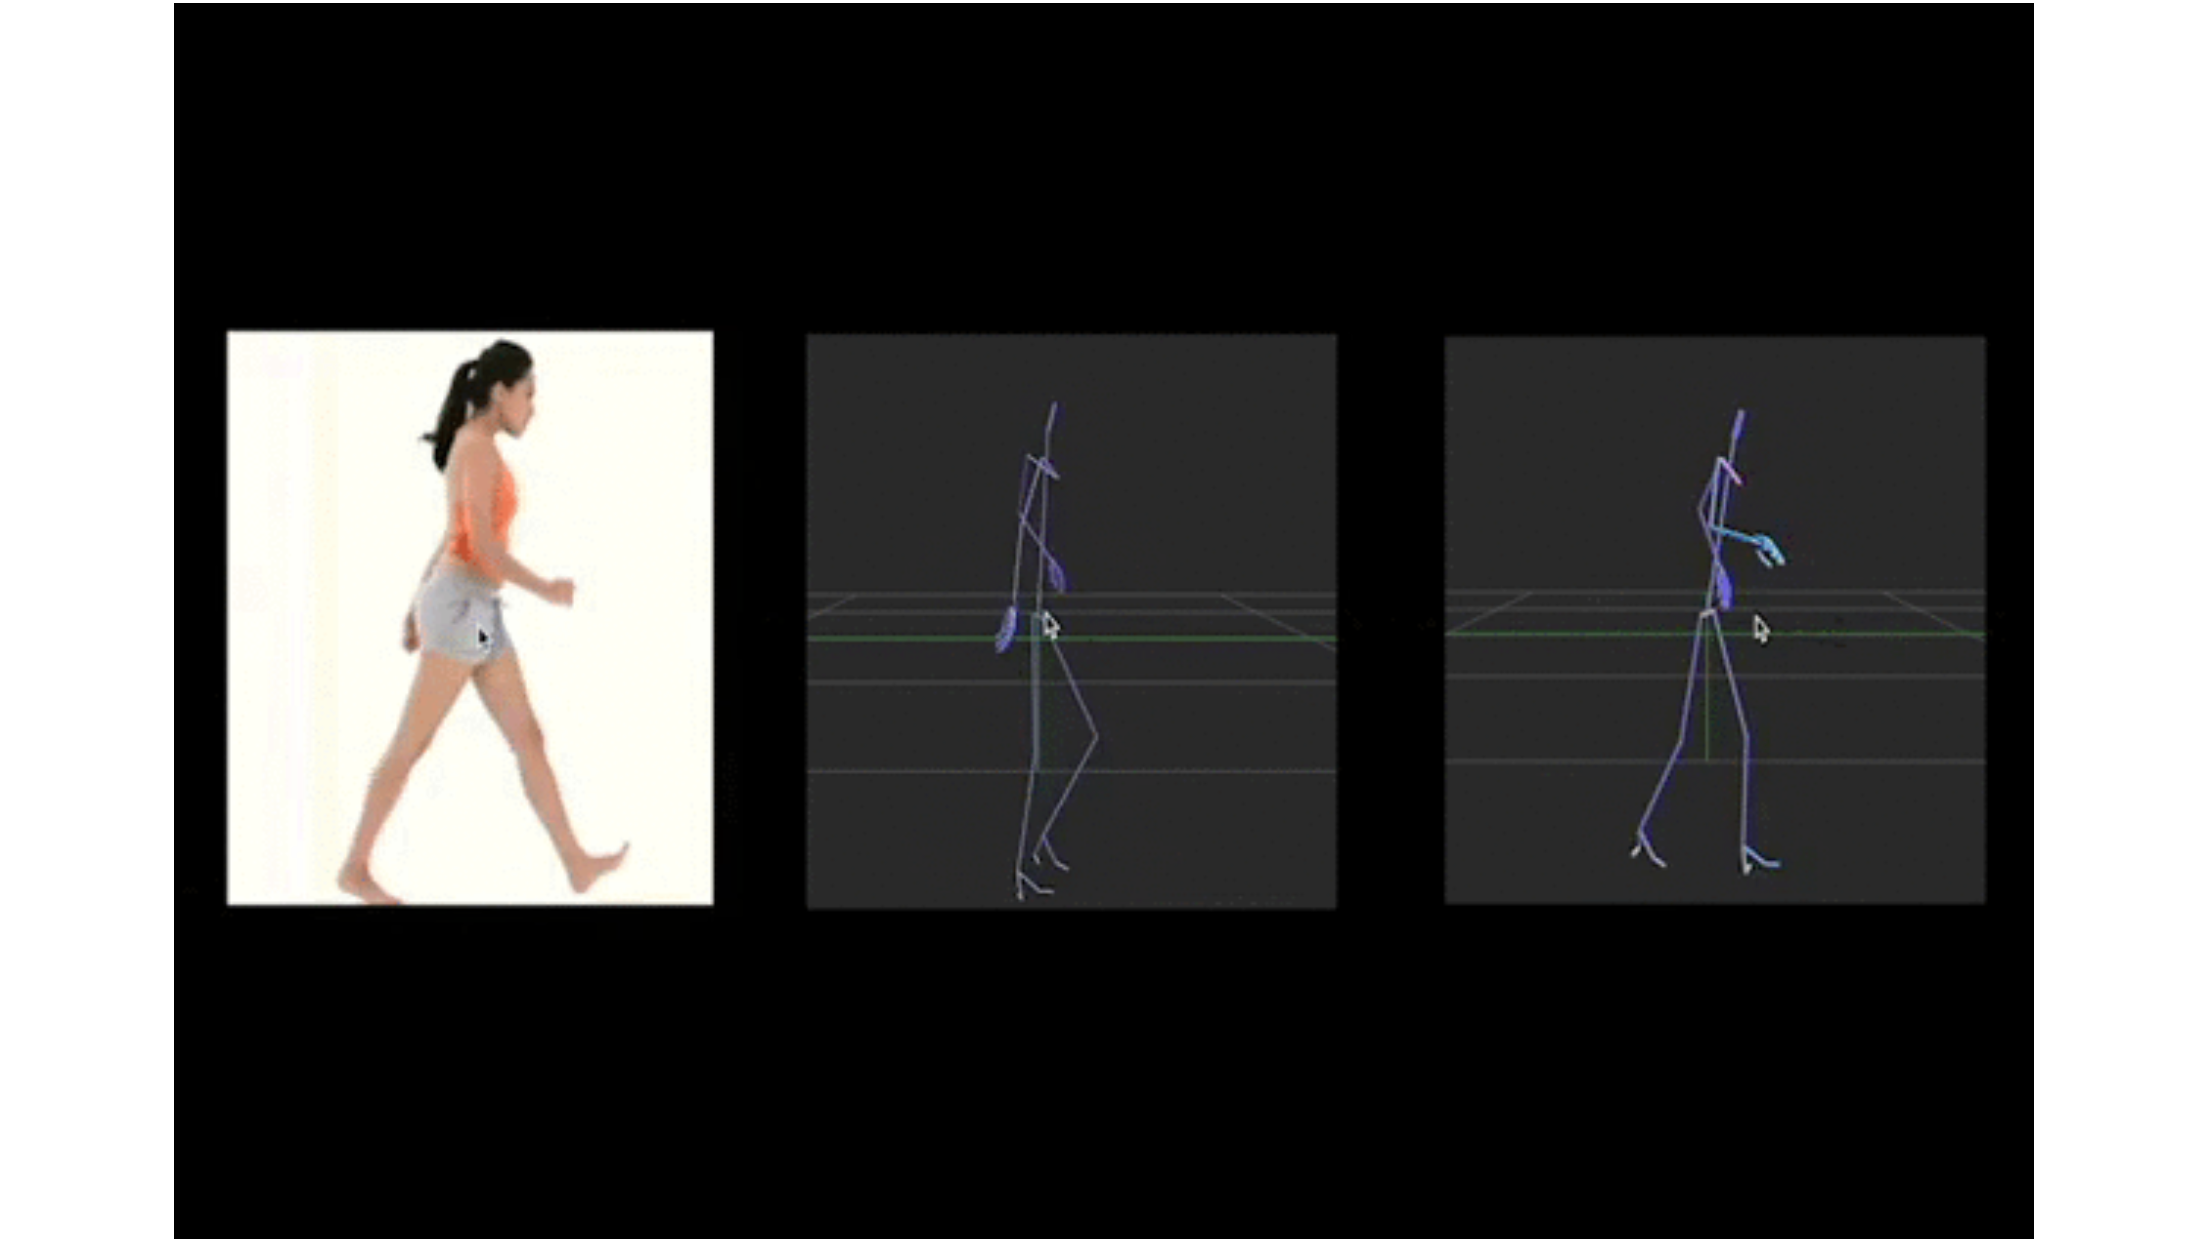
\includegraphics[width=0.3\textwidth]{2dtobvh3}
}
\caption{2D图像到BVH文件转换}
\label{fig:2dtobvh}
\end{figure}
如\cref{fig:2dtobvh}静态所示(左边为原始图片,中间为原始的姿态估计的结果\cite{kanazawa2018end},右边为运用$\mathbf{IK}$解算器修正后的图片),原始的姿态估计结果,有一些动作不符合人体骨骼活动的自然规律,例如肘关节向外翻转。但与此同时可以注意到,某一些关节,例如肩关节和腕关节,在姿态估计中的准确度远远高于肘关节这类活动范围更大的关节。所以将$\mathbf{IK}$解算器姿态估计问题中时,以右手臂为例,只考虑肩关节和腕关节的三维坐标,运用解算器反向推倒出肘关节的旋转角,然后再将其转换为世界坐标。在动态的GIF图中可以观察到,运用$\mathbf{IK}$解算器后的右手臂的弯曲更为自然。

除此之外,本文的去噪滤波器在姿态估计中也不可忽视。\cref{fig:2dtobvh}中的姿态已经经过去噪滤波器降噪处理过。在动态的GIF中,原始的姿态估计结果的抖动非常明显,甚至root关节点的世界坐标都呈现出不规律的抖动;但在运用了本文的去噪滤波器方法后,整体的运动消除了抖动,呈现出平滑效果,符合人体运动规律。


\section{讨论}{Discussion}

\subsection{不同网络结构的比较}{Comparison of Different Network Structures}
图\ref{fig:comparison_structure}验证了本文的网络选择的有效性,将其与其他流行网络进行性能比较,包括卷积神经网络(CNN),全连接神经网络(FCN)和生成性对抗网络(GAN)。这些网络的实现代码和模型在公开Github上(请参阅本文~\ref{sec:implementation}中的链接)

结果表明,具有相当小节点的RNN实现了与比其节点多的FCN相当的性能。因为RNN具有对时序序列表现更加优秀的特性,而本文中提出的对原始的数据经过额外的整合,加入了时间关联性,使之更符合RNN网络输入数据的特征要求。同时,FCN比起RNN非常可能导致过拟合问题,虽然在训练集上表现相当,但在测试集上FCN的表现远远不如RNN。在实际情况中,FCN只学习训练集的数据,相当于记忆了一个庞大的数据库,测试集上的损失函数并未明显下降,从另一方面证明FCN网络并未学习到如何求解$\mathbf{IK}$问题。

实验结果同样证明,CNN和GAN在本文的案例中不能产生令人满意的表现。CNN在实验过程,损失函数始终无法下降;GAN的调节参数过于复杂,且该问题是一个典型的监督学习问题,GAN的学习特征与之并不符合,所以GAN网络的损失函数一直无法收敛也可以得到解释。
\begin{figure}[!htbp]
	\centering
	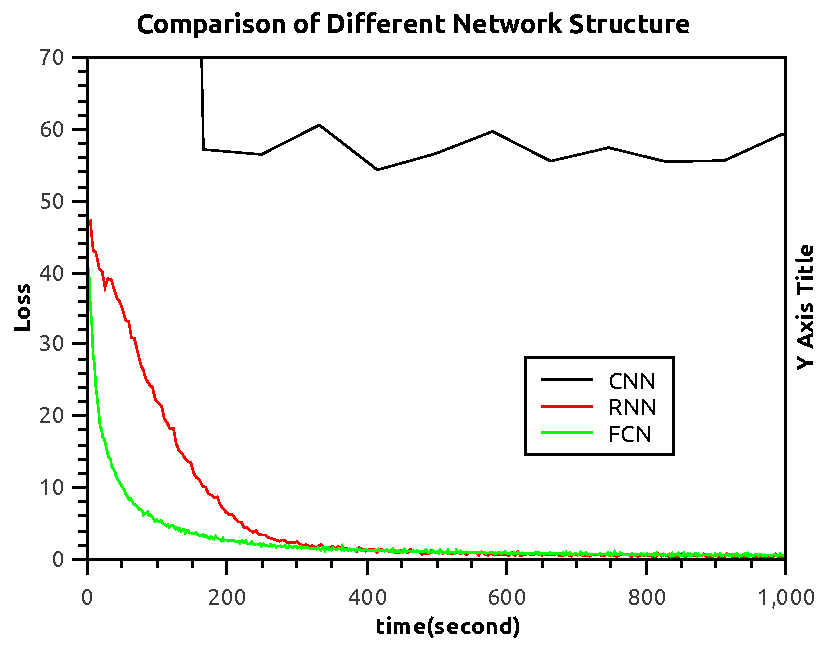
\includegraphics[width=0.75\linewidth]{comparison_structure.pdf}
	\caption[]{\label{fig:comparison_structure}
		不同网络模式的学习性能比较
	}
\end{figure}
\subsection{不同帧数输入的比较}{Comparison of Different Number of Input Frames}
\label{sec:different_nums}
\begin{figure}[!htbp]
	\centering
	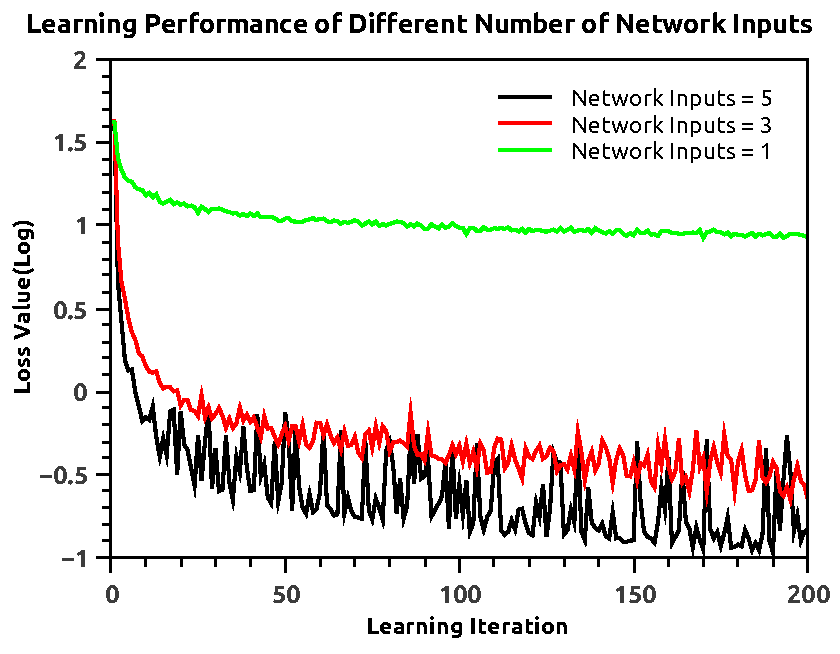
\includegraphics[width=0.75\linewidth]{comparison_num_inputs.pdf}
	\caption[]{\label{fig:comparison_num_inputs}
		不同输入帧数输入的网络学习性能比较
	}
\end{figure}
图\ref{fig:comparison_num_inputs}比较了当不同数量的帧用作网络输入时的学习性能。 该图表明,当单个帧用作网络输入时,学习性能不会产生令人满意的结果。实验中,将输入一帧的训练后的模型经过反算得到的BVH文件播放后,呈现出了巨大的抖动,且不符合人体运动规律。当增加帧数作为输入时,学习性能得到改善,但损失的方差同时也稍微更大。实验中,如\cref{fig:comparison_num_inputs2}所示,试验了输入7帧以上的结果,并没有太大的提升效果。为了学习性能、内存空间和稳定性的平衡,本文选取网络输入为5。
\begin{figure}[!htbp]
	\centering
	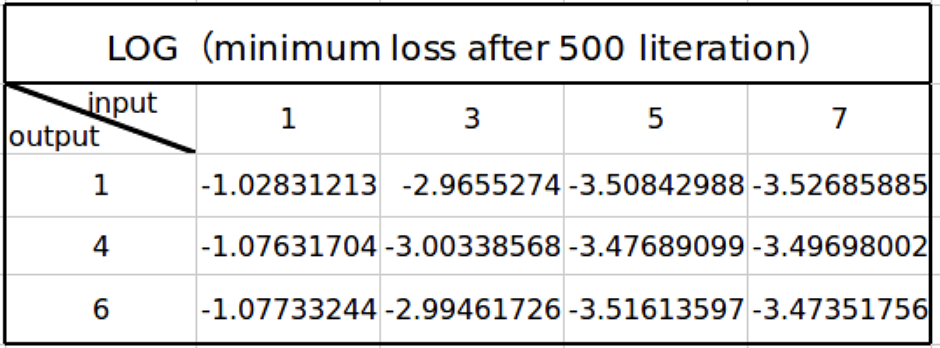
\includegraphics[width=0.75\linewidth]{comparison_num_inputs_2}
	\caption[]{\label{fig:comparison_num_inputs2}
		不同输入帧数和输出帧数的网络学习性能比较
	}
\end{figure}
\subsection{左臂和右臂的比较}{Comparison of Left and Right Arms}
图\ref{fig:comparison_left_right}比较了求解左侧手臂和右侧手臂时IK求解器的学习性能。
两种情况下的网络学习表现相似,只是左臂的函数损失相对较小且更稳定(因为损失函数做了$log$变换,将原来的细节进行了放大,实际情况中,二者差别更小一些)。这种差异应该是由于右臂负责更复杂的运动造成的(除了以左手为惯用手的少数群体)。在CMU的Mocap数据库中,经过排查后,几乎没有左撇子的参与者(考察了篮球运动类似的需要区分左右手的情况)。与左臂相比,一个以右手为惯用手的人右臂往往负责具有更高的复杂性的动作,活动范围也更大。这是导致右臂的$\mathbf{IK}$的IK解算器具有更高的函数损失和更多的抖动变化的主要原因。
\begin{figure}[!htbp]
	\centering
	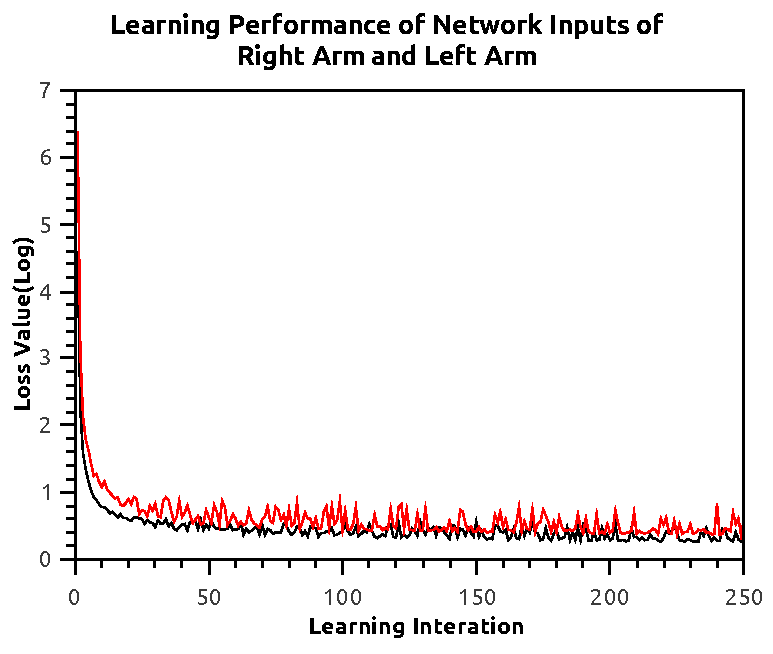
\includegraphics[width=0.75\linewidth]{comparison_left_right.pdf}
	\caption[]{\label{fig:comparison_left_right}
		左臂和右臂的网络学习性能表现
	}
\end{figure}
\subsection{手臂和腿的比较}{Comparison of Arm and Foot}
图\ref{fig:comparison_foot_arm}比较了在求解右侧的腿部和手臂的IK问题时网络的学习性能。结果表明,脚的解算器的平均损失和方差远小于手臂的平均损失和方差。这反映了一个事实,手部运动比脚部运动更加细腻和复杂。根据人类常识,手进行的活动比腿部更为复杂,且数量更多,且由于韧带和人体结构的影响,手臂的活动范围远远大于腿部。
\begin{figure}[!htbp]
	\centering
	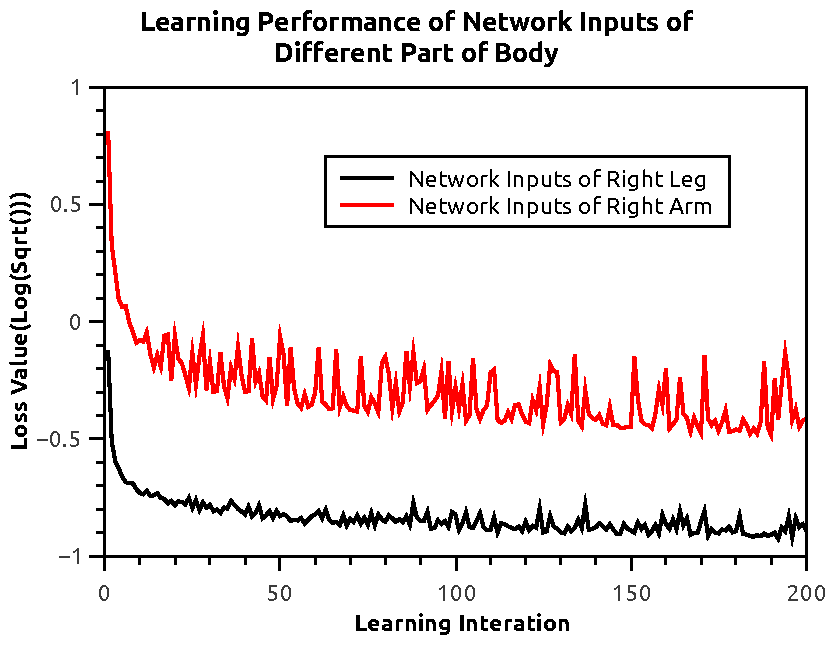
\includegraphics[width=0.75\linewidth]{comparison_foot_arm}
	\caption[]{\label{fig:comparison_foot_arm}
		手臂和腿部的网络学习性能比较
	}
\end{figure}
\subsection{重定位动作至不同肢体长度角色}{Motion Retargetting to Characters with Different Limb Lengths}
\label{sec:Retargetting}
由于末端执行器的位置用肢长度进行了标准化,以右手臂为例,
\begin{displaymath}
\overrightarrow{AC}=\frac{(\overrightarrow{AB}+\overrightarrow{BC})}{(\left|\overrightarrow{AB}\right|+\left|\overrightarrow{BC}\right|)}
\end{displaymath}
式中$\overrightarrow{AB}$、$\overrightarrow{BC}$、$\overrightarrow{AC}$皆为三维向量,分别表示右大臂、右小臂和IK解算器输入的向量.$\mathbf{A}$表示肩关节的位置,$\mathbf{B}$表示肘关节位置,$\mathbf{C}$表示腕关节位置.\cref{fig:limb_length}展示了本文方法可以推广到具有不同肢长的角色的IK问题的求解.三张图内虽然肢体长度差别巨大,但在BVH PLAYER中进行播放时,手臂和腿部的活动并未出现滑动和抖动,皆符合人体运动的规律。
\begin{figure}
\centering
\subfigure[站立动作(正常肢体长度)] {
\label{fig:standard}
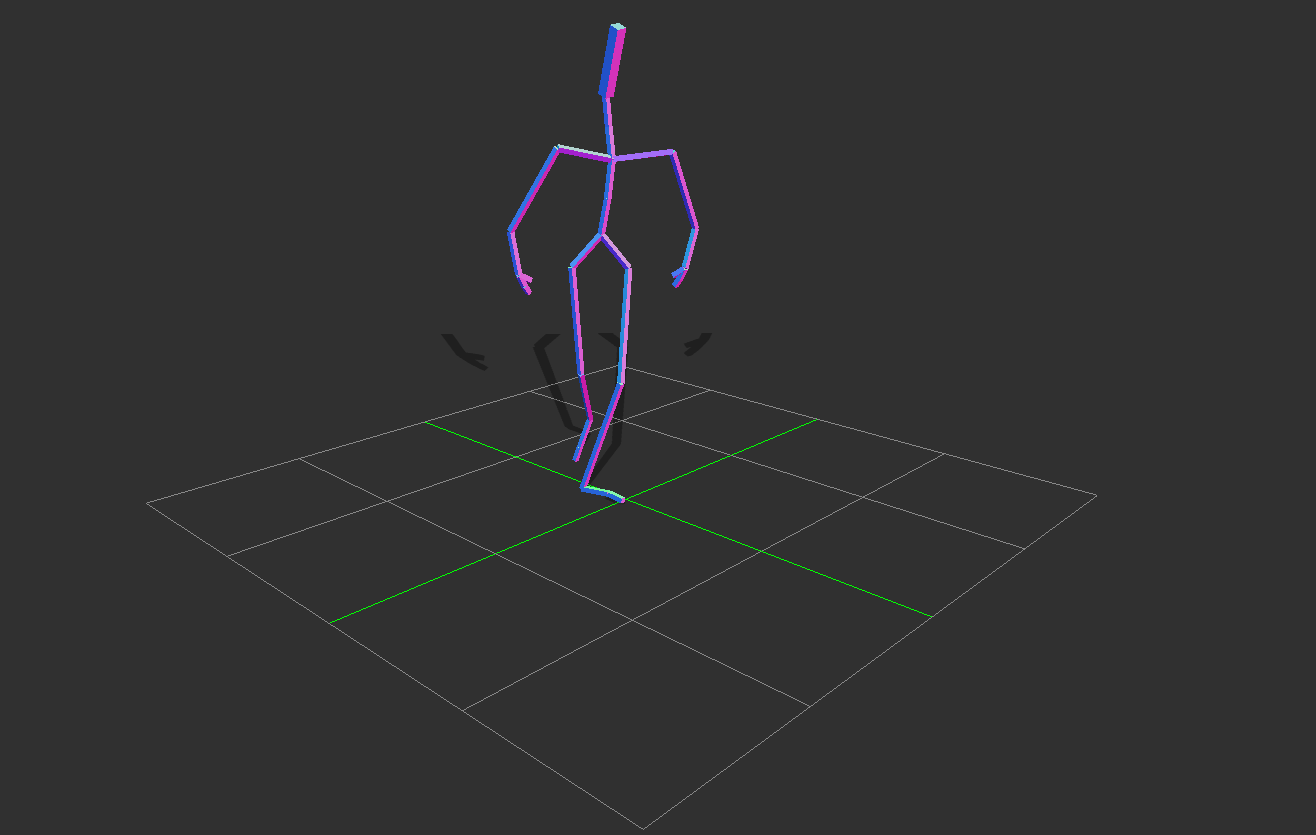
\includegraphics[width=0.3\textwidth]{standard}
}
\subfigure[站立动作(短臂)] {
\label{fig:short_arm}
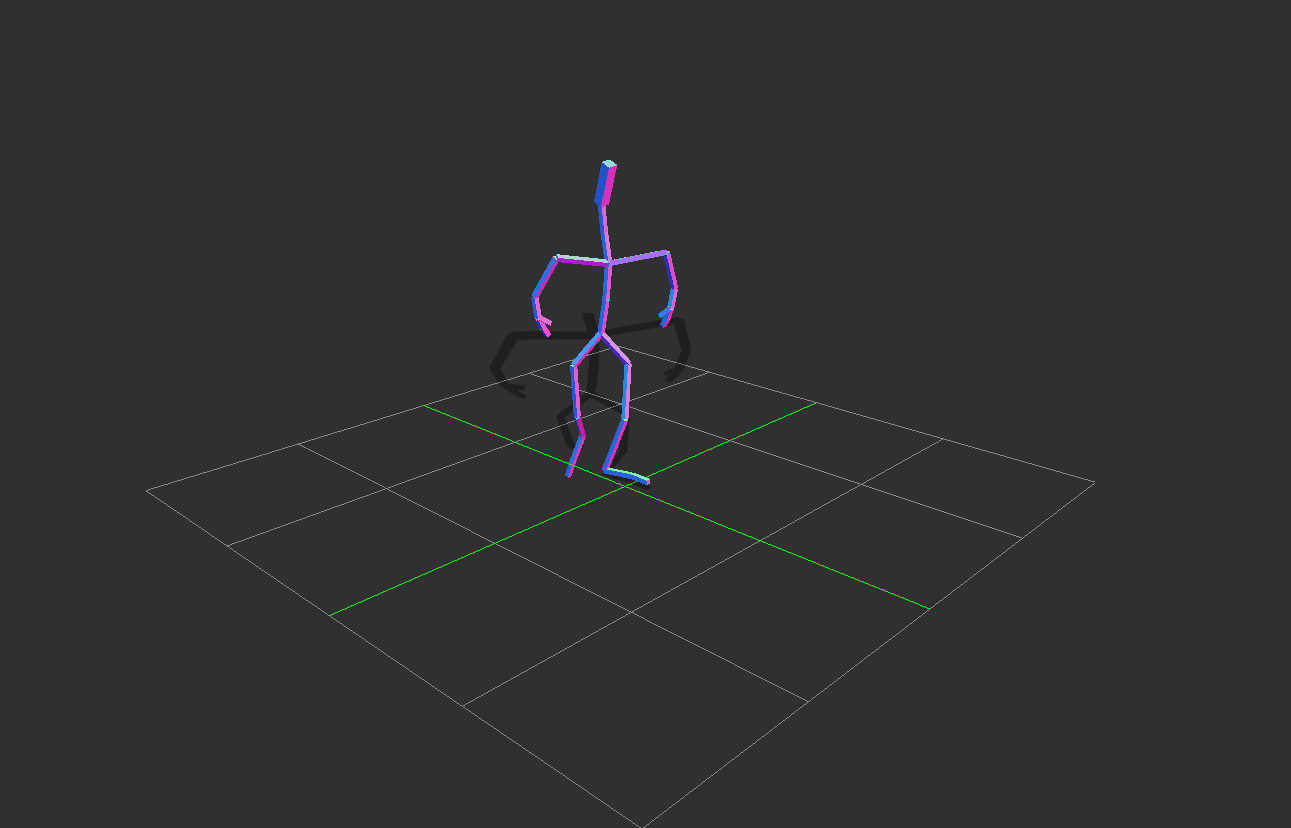
\includegraphics[width=0.3\textwidth]{short_arm}
}
\subfigure[站立动作(短腿)] {
\label{fig:short_leg}
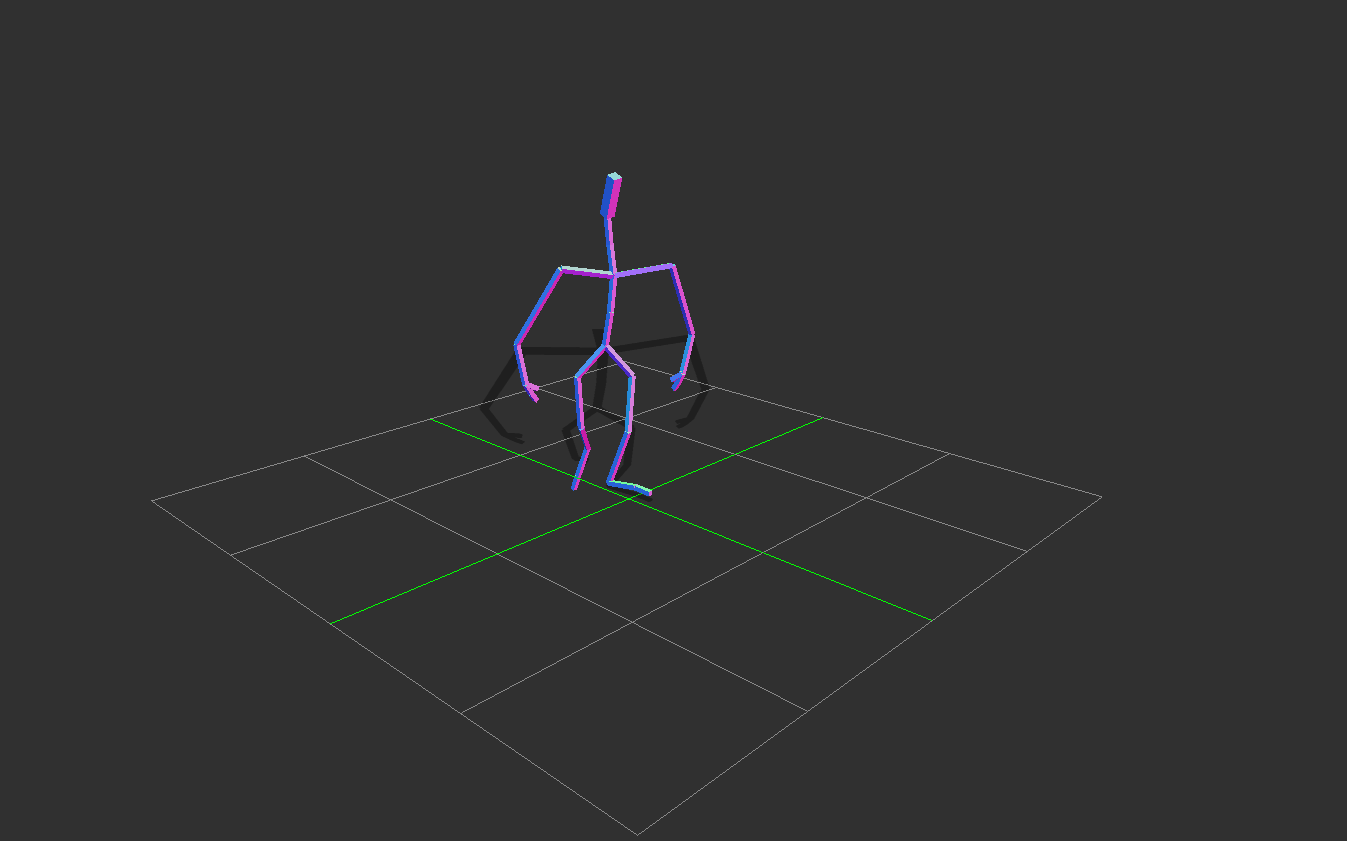
\includegraphics[width=0.3\textwidth]{short_leg}
}
\caption{不同肢体长度角色的合成动作}
\label{fig:limb_length}
\end{figure}
\section{应用}{Application}
\subsection{关键帧轨迹}{Trajectory Key-framing}
本文涉及工作的一个直接应用就是关键帧轨迹。用户将末端效应器的运动轨迹拟合为一条样条曲线,IK解算器可以自动生成沿着身体关节连接方向的各个关节角度,以获得四肢完整的关节运动轨迹。该任务首先应使用均匀参数对样条曲线进行采样,其次还需要将连续多帧合并为一段输入作为神经网络的输入。
\subsection{实时动作压缩}{Real-time Motion Compression}
本文方法的另一个应用是动作压缩。 在标准类型的动作文件(例如BVH格式)中,角色动作用根关节的全局变换和子关节相对于父关节的偏移和方向来描述。 鉴于IK求解器具有高精度,因此用末端执行器的位置替换关节的角度和方向是足够的。 这种方法可以将动作的存储空间减少至少$50\%$,这对于实时应用程序中的数据传输非常的重要。

\subsection{频繁交互环境中的运动合成}{Motion Synthesis in Contact-rich Environment}
\cref{fig:train_screenshot}和\cref{fig:test_screenshot}均展示了在涉及频繁的肢体与环境接触的情景,本文所述的方法仍具有合成自然的动作的能力。

% !TeX root = ../Main/XMU.tex
\chapter{总结}{Conclusion}
本文提出了一种利用深度学习神经网络求解IK问题的方法,特别是目前涉及此问题最为广泛的机械臂领域。此IK解算器能够处理涉及复杂人体-环境交互的场景,与此同时可以生成与真实动作最相似的骨骼姿态。本次毕业论文的主要贡献可以概括如下:
\begin{itemize}
  \item 将深度学习技术应用至该问题。不同于以往的其他论文中的工作,做到了大规模的数据集上的训练并得到了可靠的测试集结果。
  \item 定义了输入帧和输出帧之间的临界时间相关性,并将之与目前应用广泛的LSTM单元进行结合。
  \item 使用了恒定肢体比率的假设和相对坐标,消除了以往工作中的个体之间的差别性,可以真正做到无需给出肢体长度等先验信息的基础上进行IK问题的求解。
  \item 对IK问题的求解的正确性进行了定义,并对IK解算器两个组件的输出进行了降噪,且降噪结果明显。
  \item 对基于单目摄像机的3D人体骨骼工作进行了复现,并运用IK解算器和去噪滤波器对结果进行了改进。
\end{itemize}

对于未来的工作,可以分为以下X点:
\begin{itemize}
  \item 对四肢的IK解算器建立关联性(如利用树网络),做到全身的end-to-end的训练。
  \item 将其他信息(如图片语义信息)等加入网络训练中,以此来改善网络的求解自然度。
  \item 将本文的IK解算器应用于全身运动捕捉,并在末端执行器上安装惯性传感器,以此来改善合成动作的自然性。
  \item 继续其他网络的求解性,如利用强化学习来解决数据库规模问题等。
\end{itemize}


%% !TeX root = ../Main/XMU.tex
\chapter{模板的使用说明}{The usage guide of this template}

\section{使用的前提}{Prediction}

为了使用该模板,需要安装一个TeX的发行版本。可以选择Texlive或者Miktex,他们都是跨平台的。而Texlive打包了比较多的宏包,较为庞大,Miktex则是临时下载没有的宏包。这里我推荐使用Miktex。但是对于Mac,推荐使用MacTeX,它是为Mac定制的发行版本,应该比较合适。特别提醒CTeX套装无法运行该模板。关于编译方式需选择XeLaTeX,否则无法正常编译该模板。


\section{几点说明}{Some notes}

为了正确使用该模板,请按照提示安装好可使用的TeX发行版本。因为论文内容比较多,因此采取了分文件的方式来构成该文档。主文档XMU.tex的位置位于Main下,正确编译后所得的pdf文件就在这里。Figure文件夹是存放图片的文件夹,该文件夹已经加入图片文件夹的位置,插入图片是无需多加路径,直接用文件名即可。关于Setting文件夹只需要把里面的Information.tex正确填入即可。而你需要编辑的仅有Body文件夹下的文件。

该模板是在厦门大学博士学位论文模板的基础上修改得到的,因为本科论文与博士学位论文的要求差别比较的,所以定制了该模板。由于本人水平有限,因此该模板写的并不好,但是应该勉强能够满足毕业论文的要求。但是仍然可能有许多错误的地方,希望各位使用者如果能发现错误之处能够提出。可以给我法邮件或者直接在github上面提issue。欢迎大家的参与,共同完善母校的模板。

由于本人是一名理科生,对文科的同学毕业论文的额外需求可能了解不多。虽说文科生用这个模板的可能性比较小,如果有人用,有额外的需求也可以提出。

联系方式:
邮箱: \href{mailto:camusecao@gmail.com}{camusecao@gmail.com}

github项目的地址 : \href{https://github.com/CamuseCao/XMU-Undergraduate-thesis-template}{XMU-Undergraduate-thesis-template}

%% !TeX root = ../Main/XMU.tex
\chapter{正文的基本要求}{Basic requirements}

正文从另右页开始。每一章应另起页,并从奇数页开始。正文一般从引言(绪论)开始,以结论或讨论结束。引言(绪论)应包括论文的研究目的、流程和方法等。研究领域的历史回顾、文献回溯、理论分析等内容应独立成章,用足够的文字叙述。结论应包含论文的核心观点,阐述自己的创造性成果及其在本研究领域中的意义、作用,交代研究工作的局限,提出未来工作的意见和建议。

正文由于涉及的学科、选题、研究方法、结果表达方式等有很大的差异,不作统一的规定,但要求自然科学论文应提供实验数据和图片资料真实,推理正确、结论清晰;人文和社会学科的论文应把握论点正确、论证充分、论据可靠,恰当运用系统分析和比较研究的方法进行模型或方案设计,注重实证研究和案例分析。

正文一般不少于 6000 字(不含图表、程序和计算数字)。用外国语言撰写的,字数参照 4 个英文单词折算 1 个中文字数进行计数。\footnote{以上内容仅供参考,详见《厦门大学本科毕业论文(设计)规范》}


\section{学术名词}{Terminology}

\begin{itemize}
	\item  科学技术名词术语采用全国自然科学名词审定委员会公布的规范词或国家标准、部标准中规定的名称,尚未统一规定或有争议的名词术语,可采用惯用的名称。
	\item 特定含义的名词术语或新名词、以及使用外文缩写代替某一名词术语时,首次出现时应在括号内注明其含义,如:OECD(Organization for Economic Co-operation and Development)
代替经济合作发展组织。
\item  外国人名一般采用英文原名,可不译成中文,英文人名按名前姓后的原则书写。一般很熟知的外国人名(如牛顿、爱因斯坦、达尔文、马克思等)可按通常标准译法写译名。

\end{itemize}



\section{物理量名称、符号与计量}{Physical quantity name, symbol and measurement}


\begin{itemize}
	\item  论文中某一物理量的名称和符号应统一,一律采用国务院发布的《中华人民共和国法定计量单位》或者国际公认的计量单位。单位名称和符号的书写方式,应采用国际通用符号。
	\item 在不涉及具体数据表达时允许使用中文计量单位如“千克”。
	\item 表达时间使用“2014 年 6 月”,不能使用“14 年 6 月”或“2014.6”。不能使用 80 年代,而应为上世纪 80 年代或 20 世纪80 年代。表达时刻应采用中文计量单位,如“下午 3 点 10 分”,不能写成“3h10min”,在表格中可以用“3:10PM”表示。
	\item 物理量符号、物理量常量、变量符号用斜体,计量单位符号均用正体。
\end{itemize}

\section{数字}{Number }

\begin{enumerate}
	\item 无特别约定情况下,一般均采用阿拉伯数字表示。
	\item 小数的表示方法:一般情形下,小于 1 的数,需在小数点之前加 0。但当某些特殊数字不可能大于 1 时(如相关系数、比率、概率值),小数点之前的 0 可去掉,如  $ r=.26,p<.05 $  。
	\item  统计符号的格式:一般除  $ \alpha , \beta , \lambda , \epsilon \text{以及} V $ 等符号外,其余统计符号一律以斜体字呈现,如\textit{ANCOVA,ANOVA,MANOVA,N,nl,M,SD,F,p,r } 等。
\end{enumerate}


\section{公式}{Equation}

\begin{enumerate}
	\item 公式应另起一行缩略书写,居于中央(注意行首无缩进),与周围文字留足够的空间区分开。
	\item 公式的编号用英文圆括号括起,放在公式右边行末,在公式和编号之间不加虚线。子公式可不编序号,需要引用时可加编 a、b、c……,重复引用的公式不得另编新序号。公式较多时,可分章编号,但应与表格、图的编序方式统一。
	\item 较长的公式最好在等号处转行,或在运算符号(如“+”、“-”号)处转行,等号或运算符号应在转行后的行首。公式中分数线的横线,其长度应等于或略大于分子和分母中较长的一方。
\end{enumerate}

\begin{equation}
1+1=2 \label{eq1}
\end{equation}

\cref{eq1} 是大家所熟知的。我们可以用这种方式进行引用:\verb|\cref{eq1}| 。

不想要编号的公式就用这样的方式:

 \[ 2\times 2=4 \]

 行内公式就是  $ \alpha ^2= \beta $

\subsection{多行公式示例}{Multiline equation}

\begin{align}
a ={} & b + c \\
={} & d + e + f + g + h + i
+ j + k + l \notag \\
& + m + n + o \\
={} & p + q + r + s
\end{align}

\begin{equation}
\begin{aligned}
a &= b + c \\
d &= e + f + g \\
h + i &= j + k \\
l + m &= n
\end{aligned} \label{eq3}
\end{equation}

\begin{theory}[Energy–momentum relation]
The relationship of energy,
momentum and mass is
\[E^2 = m_0^2 c^4 + p^2 c^2\]
where $c$ is the light speed.
\end{theory}

\begin{law}\label{law:box}
Don’t hide in the witness box.
\end{law}


\begin{proof}
For simplicity, we use
\[
E=mc^2
\]
That’s it.
\end{proof}


\section{算法}{Algorithm}

这是算法的插入示例,可能软件学院、信息科学学院这类的同学用得上吧。

\begin{algorithm}
	\caption{My algorithm}\label{euclid}
	\begin{algorithmic}[1]
		\Procedure{MyProcedure}{}
		\State $\textit{stringlen} \gets \text{length of }\textit{string}$
		\State $i \gets \textit{patlen}$
		\BState \emph{top}:
		\If {$i > \textit{stringlen}$} \Return false
		\EndIf
		\State $j \gets \textit{patlen}$
		\BState \emph{loop}:
		\If {$\textit{string}(i) = \textit{path}(j)$}
		\State $j \gets j-1$.
		\State $i \gets i-1$.
		\State \textbf{goto} \emph{loop}.
		\State \textbf{close};
		\EndIf
		\State $i \gets i+\max(\textit{delta}_1(\textit{string}(i)),\textit{delta}_2(j))$.
		\State \textbf{goto} \emph{top}.
		\EndProcedure
	\end{algorithmic}
\end{algorithm}


\section{表格}{Table}

\begin{enumerate}
	\item 表格要有:表号,表名,单位。表号和表名居表上方正中(注意行首无缩进);表格只有一个单位时,单位在表右上方。表较多时,可分章编号,但须与插图、公式的编序方式统一。
	\item 表格应优先采用三线表,三线表头尾两条线宽 1 磅,中间线宽 0.75 磅。也可根据需要使用其他格式。
	\item 表格如参考其他资料,应标明“作者、来源名称、时间”,置表格左下方。
	\item 表格允许下页接写,接写时应重复表号,表号后跟表名(可省略)和“(续)”,置于表上方。续表应重复表头。
	\item 表格应放在离正文首次出现处最近的地方,不应超前和过分拖后。表与上下正文之间各空一行。
\end{enumerate}



\begin{table}[h!]
			\centering
	\begin{threeparttable}[b]
		\footnotesize
		\caption{表格示例}
		\begin{tabular}{lrr}
			\toprule
			& \multicolumn{1}{c}{ABS} & \multicolumn{1}{c}{CB} \\
			\midrule
			(Intercept) & 5.482 & 3.4871 \\
			ABC & 1.1173 & 1.1933 \\
			DEF & 8.1752* & 2.6836 \\
			\bottomrule
			\multicolumn{3}{c}{*p<0.1; **p<0.05; ***p<0.01} \\
			\bottomrule
		\end{tabular}%
		\label{tab:mlogit}%
		\begin{tablenotes}
			\footnotesize
			Note: These are estimates of multinomial logit model.
		\end{tablenotes}
	\end{threeparttable}
\end{table}%

%这个示例的\cref{law:box},应该是符合规定。

\section{插图}{Figure}

\begin{enumerate}
	\item 图包括曲线图、构造图、示意图、框图、流程图、记录图、地图、照片等。图应与文字内容相符,技术内容正确。所有制图应符合国家标准和专业标准,对无规定符号的图形应采用该行业的常用画法。
	\item 图要有:图号,图名,单位。图号和图名要居图下方的正中(注意行首无缩进)。图较多时,可分章编号,但须与表格、公式的编序方式统一。
	\item 图如参考其他资料,要示明“作者、来源名称、时间”,置图左下方。
	\item 由若干分图组成的插图,分图用 a、b、c……标序。分图的图名以及图中各种代号的意义,以图注形式写在图题下方,先写分图名,另起行写代号的意义。
	\item 图与图标题、图序号为一个整体,不得拆开排版为两页。当页空白不够排版该图整体时,可将其后文字部分提前,将图移至次页最前面。
\end{enumerate}

\begin{figure}[h!]
\centering

\includegraphics[scale=0.5]{xmu-flag}
\caption{Our flag} \label{fig11}
\end{figure}

这 \cref{fig11} 就是这样了。 图片等的引用都可以用 \verb|\cref{label}| 来完成。


\section{注释}{Exegesis}

当文中的字、词或短语需要进一步加以说明,而又没有具体的文献来源时,用注释。注释不宜过多。
篇名、作者注置于当页地脚。对文内有关特定内容的注释可夹在文内(加圆括号),也可排在当页地脚,注释序号以“\circled{1}、\circled{2}”等数字形式标示在被注释词条的右上角。注脚的命令如下\verb|\footnote{注脚内容}|\footnote{一个注脚}。

\section{参看文献与引用}{Reference and citation}

一下是一些参考文献的引用。应该能有合适的。不合适可以修改。


\cite{刘海洋2013latex,CTEX}

\cite{XMU}

\citet{刘海洋2013latex}

\citep{刘海洋2013latex}

\citealt{刘海洋2013latex}

\citeauthor{刘海洋2013latex}

\citeyearpar{刘海洋2013latex}


\backmatter

\addcontentsline{toc}{chapter}{参考文献 \Dotfill }
\addcontentsline{eoc}{chapter}{Reference \Dotfill }
\fancyhead[CO]{\xiaowu 参考文献}
\nocite{*}%添加此处
\wuhao
\bibliography{../Body/Reference}
%\newpage
%\appendix
%\fancyhead[CO]{\xiaowu 附录}
%\chapter*{附录}
%\addcontentsline{toc}{chapter}{附录A \Dotfill }
%\addcontentsline{eoc}{chapter}{Appendix A \Dotfill}

%下面是一个Matlab的代码的插入,还可以插入其它类型的代码。有额外需求可以添加。

\lstinputlisting[language=Matlab]{../Body/Plot.m}

附录里面还可以放其它需要的内容,它们是文章的补充。



\end{document}
